Conditionals are sentences that propose a scenario (which may or may not be the actual scenario), then go on to say something about what would happen in that scenario.\footnote{I take this framing, which emphasizes the contents of conditionals rather than their grammatical form, from \citep{fintel:conditionals}.}  In English, they are typically expressed by `if\ldots then\ldots' statements.  Examples of conditionals include:
\begin{enumerate}
\item If the Axiom of Choice is true, then every set can be well ordered.
\item You will probably get lung cancer if you smoke.
\item If the syrup forms a soft ball when you drop it into cold water, then it is between 112 and 115 degrees Celsius.
\item If kangaroos had no tails, they would topple over.
\item When I'm queen, you will be sorry.
\end{enumerate}

In general, a conditional is formed from two smaller statements: an \emph{antecedent} (the supposition that typically comes directly after `if') and a \emph{consequent} (the statement that typically comes later in the sentence, and is sometimes preceded by `then').  In the above examples, the antecedents are:
%
\begin{enumerate}
\item The Axiom of Choice is true.
\item You smoke.
\item The syrup forms a soft ball when you drop it into cold water.
\item Kangaroos had no tails.  (Or perhaps: Kangaroos have no tails.)
\item I'm queen.
\end{enumerate}
%
while the consequents are:
%
\begin{enumerate}
\item Every set can be well ordered.
\item You will probably get lung cancer.  (Or perhaps: You will get lung cancer.)
\item The syrup is between 112 and 115 degrees Celsius.
\item Kangaroos would topple over.  (Or perhaps: Kangaroos topple over.)
\item You will be sorry.
\end{enumerate}


\section{Why Care About Conditionals?}

Conditionals are useful for a variety of everyday tasks, including decision making, prediction, explanation, and imagination.

When making a decision, you should aim to choose an act such that, if you (were to) perform it, a good outcome is (or would be) likely to result.  Decision theory codifies this intuition in formal terms, and often makes explicit use of conditionals   \citep{gibbard-harper, vinci-decision, bradley-conditionals, Cantwell2013-CANCIC}.

Conditionals are also useful for deriving predictions and explanations from theoretical models.  If I am not sure which model of climate change to accept, I can use conditionals to reason about how much the earth's temperature will increase if each of the models under consideration is true.  To check whether a model explains the data I have already observed, I can use conditionals to check whether, if a given model is true, my data should be expected.  (For a defense of conditionals in scientific explanation, see \citealp{Woodward2004-WOOCAC}; for a defense of conditionals in historical explanation, see \citealp{Reiss2009-REICTE}, and \citealp{Nolan2013-NOLWHA}.)

Children's pretend play is both developmentally important, and closely related to reasoning with conditionals.  \citet{amsel-smalley}, \citet{dias-harris}, \citet{gopnik-phil-baby}, \citet{harris-imagination}, \citet{lillard-pretend}, and \citet{walton-mimesis} argue that children's pretense (for example, pretending a banana is a telephone), involves constructing an alternative scenario to what is known or believed to be true, and then reasoning about what would happen in that scenario.  While children can express their thoughts about pretend scenarios without the explicit use of conditionals, conditionals are particularly well suited to expressing these thoughts.  \citet{weisberg-gopnik} argue that the ability to reason about non-actual scenarios is crucial to learning from and planning for the actual world, since it enables children to generate and compare a range of alternative models of reality.  \citet{kryzyzanowska} argues that the mechanism that lets children evaluate conditionals is the same as the one that lets them attribute false beliefs to others.

In addition to playing a crucial role in everyday reasoning and cognitive development, conditionals do work in philosophical analyses of a variety of concepts.  Any philosophical idea that relies on the notion of dependence is ripe for a conditional analysis: to say that one thing $e$ depends on a second thing $c$ is arguably to say that if $c$ is one way, then $e$ is some corresponding way, and if $c$ is a different way, then $e$ is a correspondingly different way.  Conditionals famously appear in analyses of causation (see \citealp{menzies-sep}, and \citealp{Collins2004-COLCAC-2}, for overviews), dispositions \citep{prior-pargetter-jackson, choi-simple-reformed, choi-conditional-dispositions}, knowledge \citep{nozick-knowledge, sosa-moore}, and freedom \citep{moore-ethics, ayer-freedom}.

Finally, conditionals figure in several common patterns of reasoning, to which we now turn.

\section{Common Patterns of Reasoning}
\label{reasoning-patterns}

The following argument forms look compelling in ordinary, natural-language arguments (though we will see that all of them have putative counterexamples).  Different formal theories of conditionals yield different verdicts about which are valid.

\subsection{Modus Ponens}

Modus ponens is the inference form:\smallskip\\
\begin{tabular}{ll}
1. & If $A$, then $C$.\\
2. &$A$.\\
\hline
$\therefore$ & $C$.
\end{tabular}\\\smallskip\\
Modus ponens is one of the most central---arguably the most central---of the inference forms involving conditionals. \citet{Bobzien2002-BOBTDO-2} traces its roots back to Aristotle's hypothetical syllogisms, and through the logic of the Peripatetics and antiquity. \citet{sep-logic-india} notes that modus ponens was a common inference pattern in Pre-Classical Indian philosophy, and quotes a representative argument in which the third-century Buddhist logician Moggaliputta Tissa explicitly notes the inconsistency of simultaneously believing `if $A$, then $C$', `$A$', and `not $C$'.    \citet{ryle-ifsobecause} even advances theory of conditionals based entirely on their ability to license modus ponens: an utterance of `if $A$ then $C$' is an `inference ticket' that allows one to move from the premise $A$ to the conclusion $C$.

Despite its perennial popularity, there are apparent counterexamples to modus ponens.  One sort \citep{mcgee:mp} involves nested conditionals.  Suppose you see a fisherman with something caught in his net.  You are almost sure it is a fish, but the next likeliest option is that it is a frog.  McGee argues that you should accept the premises of the following argument, but not the conclusion (since, if the animal has lungs, then it is not a fish but a frog).\smallskip\\
\begin{tabular}{ll}
1. & If that is a fish, then if it has lungs, it's a lungfish.\\
2. & That is a fish.\\
\hline
$\therefore$ & If it has lungs, it's a lungfish.
\end{tabular}

\medskip

Another type of apparent counterexample \citep{kolodny-macfarlane, Darwall1983-DARIR} involves `ought's or `should's.  Consider this variant of Darwall's example.\smallskip\\
\begin{tabular}{p{0.03\textwidth}p{0.90\textwidth}}
1. & If you want to hurt my feelings, you should make fun of the way my ears stick out.\\
2. & You want to hurt my feelings.\\
\hline
$\therefore$ & Therefore, you should make fun of the way my ears stick out.
\end{tabular}\\\smallskip\\
Even if you do want to hurt my feelings, you shouldn't make fun of the way my ears stick out, because it's wrong to hurt my feelings.  \citet{DowellJL2011-DOWAFC-2}, and \citet{Lauer2014-LAUPND} object to the Darwall example (and other, related examples) on the grounds that they equivocate on different meanings of `should'.

Yet another type of apparent counterexample to modus ponens, discussed by \citet{walton-mp}, involves defeasible inferences, like the famous Tweety Bird example from cognitive science \citep{brewka-tweety}\smallskip\\
\begin{tabular}{ll}
1. & If Tweety is a bird, then Tweety flies.\\
2. & Tweety is a bird.\\
\hline
$\therefore$ & Tweety flies.
\end{tabular}\\\smallskip\\
The first premise of the Tweety bird argument says that there is a defeasible connection between being a bird and flying---one that can be overridden by extra information, e.g., that Tweety is a penguin.  Thus, the premises are true, and the conclusion false, in the case where Tweety is a penguin.

\subsection{Modus Tollens}

Modus tollens is the inference form:\smallskip\\
\begin{tabular}{ll}
1. & If $A$, then $C$.\\
2. &Not $C$.\\
\hline
$\therefore$ & Not  $A$.
\end{tabular}\\\smallskip\\
Modus ponens and modus tollens seem to have originated together (see \citealp{Bobzien2002-BOBTDO-2}, and \citealp{sep-logic-india}), and are closely related.  Both inferences posit a three-way inconsistency between `if $A$, then $C$', `$A$' and `not $C$'.  Affirm two of these inconsistent claims, and you'll have to deny the third.

\citet{yalcin-tollens} presents a putative counterexample to modus tollens.  Consider an urn that contains 100 marbles---some red, some blue, some big, and some small---in the following proportions.
\begin{center}
\begin{tabular}{c|cc}
& blue & red\\
\hline
big & 10 & 30\\
small & 50 & 10
\end{tabular}
\end{center}
A marble is chosen at random and placed under a cup; no other information about the situation is available.

In Yalcin's scenario, it is reasonable to accept the premises, but not the conclusion, of this instance of modus tollens.\smallskip\\
\begin{tabular}{ll}
1. & If the marble is big then it's likely red.\\
2. & The marble is not likely red.\\
\hline
$\therefore$ & The marble is not big.
\end{tabular}

\subsection{Conditional Proof}

Conditional proof (sometimes called the \emph{deduction theorem} in formal logic) lets us establish conditional conclusions without relying on any conditional assumptions.  Suppose that an argument from the premises $X$ and $A$ to the conclusion $C$ is valid.  Then conditional proof lets us conclude that the argument from $X$ to `if $A$, then $C$' is valid.  (Unlike modus ponens and modus tollens, which let us reason from the truth of some propositions to the truth of another proposition, conditional proof lets us reason from the validity of one argument to the validity of another.)

\citet{stalnaker-indicative} gives an argument that can easily be worked into a counterexample to conditional proof (though he does not present it that way).  The following argument is valid, since in classical logic, anything follows from a contradiction:\smallskip\\
\begin{tabular}{ll}
1. & The butler did it.\\
2. & The butler didn't do it.\\
\hline
$\therefore$ & The gardener did it.
\end{tabular}\\\smallskip\\
But the following argument is not valid:\smallskip\\
\begin{tabular}{ll}
1. & The butler did it.\\
\hline
$\therefore$ & If the butler didn't do it, then the gardener did it.
\end{tabular}

\medskip

Although conditional proof in its full generality looks implausible, a restricted version is more appealing: if $A$ all by itself entails $C$, then `if $A$, then $C$' is a truth of logic.  (\citet{koons-sep}  makes a similar suggestion about conditional proof in nonmonotonic logic.)

\subsection{Transitivity, Contraposition, and Strengthening the Antecedent}
\label{strengthening}

Transitivity is the inference form:\smallskip\\
\begin{tabular}{ll}
1. & If $A$, then $B$.\\
2. & If $B$, then $C$.\\
\hline
$\therefore$ & If $A$, then $C$.
\end{tabular}\\\smallskip\\
Contraposition is:\smallskip\\
\begin{tabular}{ll}
1. & If $A$, then $C$.\\
\hline
$\therefore$ & If not $C$, then not $A$.
\end{tabular}\\\smallskip\\
And strengthening the antecedent is:\smallskip\\
\begin{tabular}{ll}
1. & If $A$, then $C$.\\
\hline
$\therefore$ & If $A$ and $B$, then $C$.
\end{tabular}

\medskip

All three inference forms seem to fail for ordinary conditionals in English.  For transitivity, we have the following counterexample \citep[106]{stalnaker:conditionals}:\smallskip\\
\begin{tabular}{p{0.03\textwidth}p{0.9\textwidth}}
1. & If J. Edgar Hoover had been born a Russian, then he would have been a communist.\\
2. & If J. Edgar Hoover had been a communist, then he would have been a traitor.\\
\hline
$\therefore$ & If J. Edgar Hoover had been born a Russian, then he would have been a traitor.
\end{tabular}\\\smallskip\\
For contraposition, we have the following counterexample \citep[adapted from][]{adams:tollens}:\smallskip\\
\begin{tabular}{ll}
1. & If it rains, then it does not rain hard.\\
\hline
$\therefore$ & If it rains hard, then it does not rain.
\end{tabular}\\\smallskip\\
And for strengthening the antecedent, we have the following counterexample \citep[106]{stalnaker:conditionals}:\smallskip\\
\begin{tabular}{p{0.03\textwidth}p{0.9\textwidth}}
1. & If this match were struck, then it would light.\\
\hline
$\therefore$ & Therefore, if this match had been soaked in water overnight and it were struck, then it would light.
\end{tabular}

\medskip

Not everyone accepts these putative counterexamples as genuine.  \citet{Brogaard2008-BROCAC} argue that the meaning of a conditional depends partly on a contextually determined set of relevant possible worlds.  They claim that the putative counterexamples involve a context shift between the premises and the conclusion, but in any fixed context, the arguments are valid.

\citet{fintel-dynamic}, \citet{Gillies2007-GILCS}, and \citet{Williams2008-WILCAC-2} cite linguistic evidence in support of the context shift hypotheses: changing the order of the premises and conclusions in the counterexample arguments changes whether they seem true or false. Counterexamples to antecedent strengthening are closely related to so-called \emph{Sobel sequences} (named for \citealt{Sobel1970-SOBUSA}).  A Sobel sequence consists of two sentences of the following form \citep{Gillies2007-GILCS}.
\begin{enumerate}
\renewcommand{\labelenumi}{(\alph{enumi})}
\item If Sophie had gone to the New York Mets Parade, she would have seen Pedro Mart\'inez.
\item But if Sophie had gone to the New York Mets Parade and gotten stuck behind a tall person, she would not have seen Pedro Mart\'inez.
\end{enumerate}
It seems perfectly reasonable to assert (a) followed by (b).  But once someone has asserted (b), an assertion of (a) seems inappropriate---after all, if Sophie had gone to the parade, who's to say she would not have gotten stuck behind a tall person?

Fintel, Gillies, and Williams claim that Sobel sequences involve a context shift: once someone asserts (b), the context changes to make (a) false, but (a) and (b) are never true in the same context.   \citet{Moss2012-MOSOTP} proposes an alternative explanation: once (b) has been asserted, (a) might be true, but is no longer known, since asserting (b) changes the standards a belief must meet in order to count as knowledge.

\subsection{Simplification of Disjunctive Antecedents}

Simplification of disjunctive antecedents (`simplification' for short; \citealp{Nute1975-NUTCAT-2}) is the argument form:\smallskip\\
\begin{tabular}{ll}
1. & If $A$ or $B$, then $C$.\\
\hline
$\therefore$ & If $A$, then $C$.
\end{tabular}\\\smallskip\\
Simplification seems appealing on its face: surely, to say that the bus will be late if it rains or snows is to say that the bus will be late if it rains, and the bus will be late if it snows.

However, one can easily generate counterexamples by substituting the same sentence for $B$ and $C$.  Suppose I have enough money to visit either Disneyland or Graceland, but not enough to visit both.  Then the premise of the following argument is true, while its conclusion is false.\smallskip\\
\begin{tabular}{ll}
1. & If I visit Disneyland or I visit Graceland, then I'll visit Graceland.\\
\hline
$\therefore$ & If I visit Disneyland, then I'll visit Graceland.
\end{tabular}

\medskip

Counterexamples to strengthening the antecedent can be used to generate counterexamples to simplification \citep{Fine1975-FINCN-2}.  Suppose we have both of the following:
\begin{enumerate}
\item If $A$, then $C$.
\item Not: if $A$ and $B$, then $C$.
\end{enumerate}
$A$ is logically equivalent to [($A$ and $B$) or ($A$ and not $B$)], so by 1, we have:
\begin{enumerate}
\item[3.] If [($A$ and $B$) or ($A$ and not $B$)], then $C$.
\end{enumerate}
But by simplification, the truth of 3 would have to entail the falsity of 2.

So there is a three-way tension between the validity of simplification, the invalidity of strengthening the antecedent, and the substitution of logical equivalents. All three ways out of the puzzle are represented in the literature: \citet{Loewer1976-LOECWD} and \citet{Mckay1977-MCKCWD} reject simplification; defenders of strict conditional accounts (\autoref{strict}) accept strengthening the antecedent; and \citet{Nute1975-NUTCAT-2} and \citet{Alonso-Ovalle2009-ALOCCA} reject substitution.

\section{The Indicative/Counterfactual Distinction}
\label{indicative-counterfactual}

Conditionals in English can be divided into two categories, exemplified by the following pair of sentences \citep{adams:subjunctive}:
\begin{description}
\item[(DD)] If Oswald did not shoot Kennedy, then someone else did.
\item[(HW)] If Oswald had not shot Kennedy, then someone else would have.
\end{description}
Although \spacedlowsmallcaps{(DD)} and \spacedlowsmallcaps{\spacedlowsmallcaps{(HW)}} are built up from the same antecedent and consequent, they mean different things. \spacedlowsmallcaps{(DD)} would be acceptable to most people familiar with US history: Kennedy was shot, so someone must have shot him---if not Oswald, then someone else.  But \spacedlowsmallcaps{(HW)} is more controversial; it is accepted by conspiracy theorists, but rejected by those who believe that Oswald acted alone.  Sentences like \spacedlowsmallcaps{(DD)} are called \emph{indicative}; sentences like \spacedlowsmallcaps{(HW)} are called \emph{counterfactual} (or sometimes \emph{subjunctive}).

It's not clear how to classify conditionals whose antecedents concern the future.  Consider the following sentence, as uttered by a conspirator before the Kennedy assassination.
\begin{description}
\item[(DW)] If Oswald does not shoot Kennedy, then someone else will.
\end{description}
\citet{dudman-tense-article, dudman-parsing} and \citet{bennett-phlogiston} argue that future-tensed conditionals like \spacedlowsmallcaps{(DW)} belong with counterfactuals like \spacedlowsmallcaps{(HW)}; Bennett (\citeyear{Bennett2003-BENAPG, bennett-explanations}; yes the same Bennett!) argues that they belong with indicatives like \spacedlowsmallcaps{(DD)}; \citet{edgington-conditionals} argues that there exist distinct categories of future-tensed indicatives and future-tensed counterfactuals.

Philosophers also disagree about the precise relationship between indicatives and counterfactuals.  Some favor what \citet{Bennett2003-BENAPG} calls `Y-shaped analyses', which first explain what is common to indicatives and counterfactuals, and then bifurcate to explain how this common core can produce two different kinds of conditionals.  Others (notably \citealp{Gibbard1981-GIBTRT}, and \citealp{Bennett2003-BENAPG}) argue that we need completely separate theories of indicatives and counterfactuals---that there is no interesting core shared by both.

In what follows, I will write `$A \boxright C$' to indicate a counterfactual conditional; `$A \rightarrow C$' to abbreviate an indicative conditional; and `if $A$, then $C$' where I wish to remain neutral.  I turn now to a popular class of theories, typically aimed at explaining counterfactual conditionals, but sometimes extended to cover indicatives.


\section{Selection Functions}

One way to give a theory of conditionals is to spell out their \emph{truth conditions}, i.e., the circumstances under which they are true.  Formally, philosophers represent the truth conditions of a sentence as a function from possible worlds (i.e., ways the world might be) to truth values.  Fully specifying the truth conditions for every conditional would be too tall an order: to understand the truth conditions for `if ontogeny recapitulates phylogeny, then snakes develop vestigial legs', we would have to understand the truth conditions of `ontogeny recapitulates phylogeny' and `snakes develop vestigial legs', and that job falls outside the scope of a theory of conditionals.  So theories of conditionals adopt a more modest aim: to give a recipe for deriving the truth conditions for `if $A$, then $C$' from the truth conditions of (arbitrary) $A$ and $C$.

The concept of a selection function \citep{stalnaker:conditionals} provides a way of assigning truth conditions to a conditional based on the truth conditions of its antecedent and consequent.  The basic idea is that, to evaluate `if $A$, then $C$', we should first consider a set of \emph{selected} possible worlds where $A$ is true.  (Henceforth, I will use `$A$-worlds' as shorthand for `worlds where $A$ is true'.)    Intuitively, the selected worlds represent ways the actual world might be if $A$ were true.  We then check whether, at all the selected worlds, $C$ is true.  If so, then the counterfactual conditional `if $A$, then $C$' is true at the actual world; otherwise, it is false at the actual world.

More formally, we can model this process in terms of a selection function $f$ that maps ordered pairs consisting of a possible world and a proposition onto sets of possible worlds.  `If $A$, then $C$' is true at a possible world $w$ if and only if $C$ is true at every world in $f(A, w)$. Different ways of interpreting the selection function yield different theories of conditionals.

\subsection{Strict Conditionals}
\label{strict}

One natural way to interpret the selection function is to check \emph{all} possible $A$-worlds, and say that `if $A$, then $C$' is true at world $w$ just in case $C$ is true at all of them.  (Since what is possible may depend on what is actual, the truth value of the conditional may vary from world to world.)  This approach yields the \emph{strict conditional} interpretation of the selection function, first developed by \citet{lewis-survey}.  The strict conditional approach classifies transitivity, contraposition, and antecedent-strengthening as valid---which its opponents claim is a mistake \citep[see][4--12]{lewis-counterfactuals}.

The strict conditional interpretation also gives questionable results about which counterfactuals are true.  If I were to leap out of the second-story window of my office, I would hurt myself---but the strict conditional account says this is not so.  There are possible worlds where I leap out the second-story window and remain unharmed: some where there is a safety net underneath the window, some where I am thoroughly ensconced in protective bubble wrap, some where my body is much less fragile than ordinary human bodies, some where the Earth's gravitational field is weak\ldots but none of them is the sort of world that would result, if I were to leap out the second-story window.  \citet{HajekManuscript-HJEMCA} sums up the problem this way: on the strict conditional interpretation, most counterfactuals are false.\footnote{H\'{a}jek argues that the problem extends beyond strict conditional accounts; it also affects the closest-worlds account in \autoref{closest}.  \citet{Lewis2015-LEWEC} argues that we can save the closest-worlds account by ignoring worlds that are deemed irrelevant by a contextually-determined standard of relevance.}

\subsection{Closest Worlds}
\label{closest}

An alternative to the strict conditional approach, typically used for counterfactuals, defines the selection function in terms of similarity among possible worlds.  For every world $w$, we can rank worlds from most similar to $w$ (`closest') to least similar (`farthest away').  \citet{lewis-counterfactuals} holds that every such ranking is a \emph{total preorder}: two worlds can be equally similar to $w$, but they must be comparable, so that either they are equally similar or one is more similar than the other.  (\citealp{stalnaker:conditionals}, discusses the special case of the logic where no two worlds are equally close to each other; \citealp{Pollock1976-POLTPW}, discusses a generalization where worlds may be incomparable in terms of closeness.)  $A \boxright C$ is true at $w$ just in case $C$ is true at all the $A$-worlds that are most similar to $w$.

Formally, the closest-worlds interpretation can be modeled using a system of `spheres'---sets of worlds such that every world in the set is closer to $w$ than every world outside it \citep{lewis-counterfactuals}. Then $f(A, w)$ is the intersection of the set of $A$-worlds with the smallest sphere containing at least one $A$-world.\footnote{Some technical difficulties arise when there is no smallest sphere containing at least one $A$-world, but only a limitless sequence of ever-smaller spheres; see \citet[424--425]{Lewis1973-LEWCAC}; \citet[96--99]{Stalnaker1981-STAADO-4}; \citet{Warmbrod1982-WARADO}; and \citet{Diez2015-DEZCTD} for discussion.}

Unlike the strict conditional interpretation, the closest-worlds interpretation of the selection function can explain why transitivity, contraposition, and antecedent-strengthening seem invalid.  On the closest-worlds interpretation, they \emph{are} invalid, and we can use diagrams (adapted from \citealp{lewis-counterfactuals}) to illustrate why.

To see why transitivity is invalid, consider a system of spheres model centered on a particular world $w$, depicted in \autoref{fig-transitivity}.  (Worlds are points in the diagram, and spheres are concentric circles.)  The $A$-worlds are the points inside the shape labeled $A$, the $B$-worlds are the points inside the shape labeled $B$, and the $C$-worlds are the points inside the shape labeled $C$.  All the closest $A$-worlds to $w$ are $B$-worlds, and all the closest $B$-worlds are $C$-worlds; yet none of the closest $A$-worlds are $C$-worlds.  \autoref{fig-contraposition} shows a counterexample to contraposition, and \autoref{fig-strengthening} shows a counterexample to antecedent strengthening.

\begin{figure}
\centering
\begin{subfigure}{0.5\textwidth}
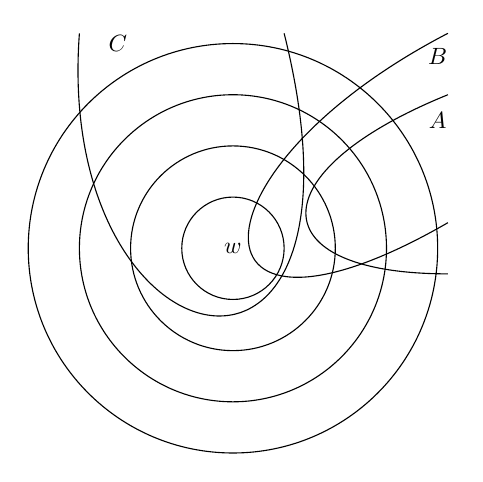
\begin{tikzpicture}[scale = 0.65, every node/.style={scale=0.85}]
\draw (0, 0) node {$w$};

\draw (0, 0) circle (1cm);

\draw (0, 0) circle (2 cm);

\draw (0, 0) circle (3cm);
\draw (0, 0) circle (4cm);


\draw (4.2, 3) .. controls (0.5, 1.5) and ( 0.5, -0.5) .. (4.2, -0.5);
\draw (4, 2.5) node {$A$};

\draw (4.2, 4.2) .. controls (-1, 1.5) and ( -1, -2.5) .. (4.2, 0.5);
\draw (4, 3.75) node {$B$};
\draw (-3, 4.2) .. controls (-3.5, -2.5) and ( 3, -3.8) .. (1, 4.2);
\draw (-2.25, 4) node {$C$};

\end{tikzpicture}
\caption{Transitivity}
\label{fig-transitivity}
\end{subfigure}

\begin{subfigure}{0.5\textwidth}
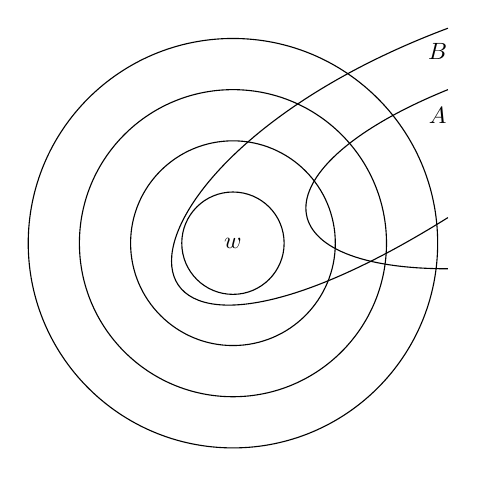
\begin{tikzpicture}[scale = 0.65, every node/.style={scale=0.85}]
\draw (0, 0) node {$w$};

\draw (0, 0) circle (1cm);

\draw (0, 0) circle (2 cm);

\draw (0, 0) circle (3cm);
\draw (0, 0) circle (4cm);


\draw (4.2, 3) .. controls (0.5, 1.5) and ( 0.5, -0.5) .. (4.2, -0.5);
\draw (4, 2.5) node {$A$};

\draw (4.2, 4.2) .. controls (-3, 1.5) and ( -3, -4) .. (4.2, 0.5);
\draw (4, 3.75) node {$B$};


\end{tikzpicture}
\caption{Contraposition}
\label{fig-contraposition}
\end{subfigure}

\begin{subfigure}{0.5\textwidth}
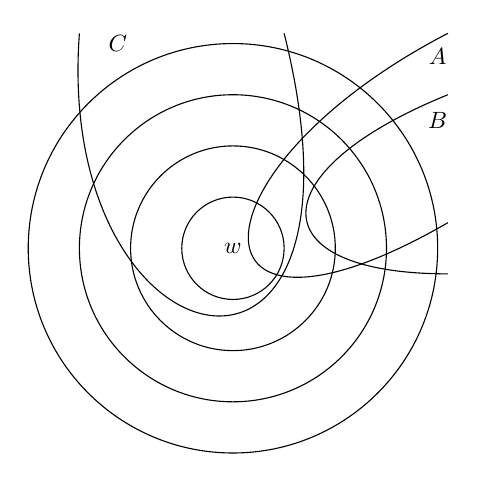
\begin{tikzpicture}[scale = 0.65, every node/.style={scale=0.85}]
\draw (0, 0) node {$w$};

\draw (0, 0) circle (1cm);

\draw (0, 0) circle (2 cm);

\draw (0, 0) circle (3cm);
\draw (0, 0) circle (4cm);


\draw (4.2, 3) .. controls (0.5, 1.5) and ( 0.5, -0.5) .. (4.2, -0.5);
\draw (4, 2.5) node {$B$};

\draw (4.2, 4.2) .. controls (-1, 1.5) and ( -1, -2.5) .. (4.2, 0.5);
\draw (4, 3.75) node {$A$};
\draw (-3, 4.2) .. controls (-3.5, -2.5) and ( 3, -3.8) .. (1, 4.2);
\draw (-2.25, 4) node {$C$};

\end{tikzpicture}
\caption{Strengthening the antecedent}
\label{fig-strengthening}
\end{subfigure}
\caption{Counterexamples to transitivity, contraposition, and strengthening the antecedent in the closest-worlds framework}
\end{figure}

Defenders of the closest-worlds theory have the burden of spelling out what `closeness' amounts to. \citet{lewis-counterfactuals} claims that closeness is based on similarity among worlds: to say that one world is closer to $w$ than another is to say that the first world is more similar to $w$ than the second.  But \citet{Fine1975-FINCN-2} presents an example where greater similarity does not make for greater closeness.  (I have taken a few liberties with the details of the example.)

On September 26, 1983, at the height of the Cold War, a Soviet early-warning system went off, falsely reporting that missiles had been launched at Russia from the US \citep{petrov}.  The officer who saw the alarm, Stanislav Petrov, did not report it to his superiors, and so Russia did not launch missiles in retaliation. The following conditional seems true:
\begin{description}
\item[PETROV] If Petrov had informed his superiors at the time of the false alarm, then there would have been a nuclear war.
\end{description}
%
After all, Petrov's superiors were poised to launch the missiles in the event of an attack, and it seems that the phone lines and missile system were in working order.  The only missing ingredient was the report from Petrov.

But among the worlds where Petrov informs his superiors at the time of the false alarm, those where the Soviet missile launch is prevented by a happy accident---incompetence by Petrov's superiors, or a broken telephone, or a malfunction of the Soviet missile system---are more similar to the actual world than those where the launch goes through.  Worlds where the missile launch is prevented by a happy accident agree with the actual world about the total number of nuclear wars in the 20th Century---surely a more important dimension of similarity than the functioning or malfunctioning of one measly telephone line.\footnote{Defenders of the closest-worlds interpretation reply that we should understand `similarity' so that agreeing about the total number of nuclear wars in the 20th Century does not make for greater similarity than agreeing about the functioning or malfunctioning of one measly telephone line; see \citet{Lewis1979-LEWCDA} and \citet{Arregui2009-ARROSI}.}

\subsection{Past Predominance}

To handle the \textsc{petrov} example, a natural thought goes, we need an account of the selection function that treats the past differently from the future. When Petrov made his choice, the missile launch system was already in working order---but it was not yet determined whether there would be a war.

\citet{Thomason1980-THOATO-4} propose an account of the selection function that takes seriously the past-future asymmetry.  They model the universe using branching time, where each moment has only one possible past, but multiple possible futures.  (\citealp{Cross1990-CROTNA}, shows that the assumption of branching time is dispensable; past predominance can also be modeled using ordinary possible worlds.)  \autoref{fig-branching-time} depicts such a model. The nodes $t_1$, $t_2$, \ldots, $t_9$ are moments.  Paths through the tree---in this example, $\{t_1, t_2, t_4, t_7\}$, $\{t_1, t_2, t_5, t_8\}$, and $\{t_1, t_3, t_6, t_9\}$---are called \emph{histories}.

\begin{figure}
\centering
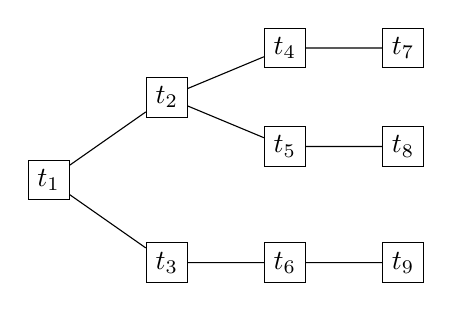
\begin{tikzpicture}[grow=right,
		level 1/.style={sibling distance=2.1cm},
		level 2/.style={sibling distance=1.25cm},
		level 3/.style={sibling distance = 0.75cm},]

\node[draw]{$t_1$}
		child{node[draw]{$t_3$}
			child{node[draw]{$t_6$}
							child{node[draw]{$t_9$}}
		}}
		child{node[draw]{$t_2$}
			child{node[draw]{$t_5$}
				child{node[draw]{$t_8$}}
			}
			child{node[draw]{$t_4$}
				child{node[draw]{$t_7$}}
				}};
\end{tikzpicture}
\caption{A model of branching time}
\label{fig-branching-time}
\end{figure}

We can think of each possible world as containing information about which moment is present, as well as information about which history is actual.  (On this way of understanding the model, even when the present moment has more than one possible future, there is a fact of the matter about which future will occur.)

Thomason and Gupta adopt a \emph{past predominance} principle, which says that if a world $x$ is in $f(A, w)$, then it must diverge from $w$ as late as possible---there can be no other $A$-world whose history overlaps $w$ for a longer span than $f(A, w)$.\footnote{For technical reasons, Thomason and Gupta also assume that $f(A, w)$ is a singleton set, and posit that each world contains a \emph{choice function}, which specifies not just what the future will be like, but what the future would have been like had the past gone differently.  I pass over the details.}

The past predominance view can explain the \textsc{petrov} example.  Consider the following interpretation of our diagram: the actual history is $\{t_1, t_2, t_4, t_7\}$. At $t_1$, it is not yet settled whether the early warning system goes off.  The early warning system goes off $t_2$, and Petrov must decide what to do.  (At $t_3$, which belongs to an alternative history, there is never any alarm.)  At $t_4$, Petrov decides not to notify his superiors, and so at $t_7$, there is no nuclear war.  (At $t_5$, which belongs to another alternative history, Petrov decides to notify his superiors, and a nuclear war ensues at $t_8$.)

Now consider the conditional \textsc{petrov}, as uttered at $t_7$.  Its antecedent is false at the actual world, which has the history $\{t_1, t_2, t_4, t_7\}$.  The closest worlds where its antecedent is true must have the history $\{t_1, t_2, t_5, t_8\}$, which diverges from the actual world's history at the last possible moment yet still makes the antecedent true.  Since the actual present moment is $t_7$, it seems reasonable to select $t_8$ as the present moment at all the closest worlds. Since there is a nuclear war at $t_8$, the consequent of \textsc{petrov} is true at all the the closest worlds; hence \textsc{petrov} is true at the actual world.


\subsection{Causal Models}

A class of examples called \emph{Morgenbesser cases} \citep[27n]{slote-counterfactuals} suggest that the selection function should respect causal as well as temporal constraints.   \citet{Edgington2004-EDGCAT} gives a representative Morgenbesser case.

Our heroine misses a flight to Paris due to a car breakdown.  She complains to the repairman: `If I had caught the plane, I would have been halfway to Paris by now!'  But he corrects her: `I was listening to the radio.  It crashed.  If you had caught that plane, you would be dead by now.'

The repairman claims that the following counterfactual is true.
\begin{description}
\item[LETHAL] If the heroine had caught that plane, she would be dead by now.
\end{description}
He is right.  It's not clear that past predominance can explain why he's right: the plane crash occurs after our heroine would have made her flight.\footnote{But see \citet{Phillips2007-PHIMCA} for an argument that past predominance \emph{can} provide an adequate explanation.}  What matters is that the plane crash is causally independent of whether she makes her flight.  This is why, when assessing what would have happened if our heroine had made her flight, we should hold the plane crash fixed.

 \citet{pearl-causality} proposes a causal theory of counterfactuals that accounts for Morgenbesser cases.  His theory relies on the concept of a \emph{causal model}, consisting of a set of \emph{variables}, which represent what circumscribed parts of the world are like, and a set of \emph{structural equations}, which represent direct causal links between variables.  Each variable is assigned an \emph{actual value}; we can think of variables as questions about parts of the world, their possible values as possible answers to those questions, and their actual values as the correct answers in the actual world.  Note that although I introduced selection semantics as a recipe for assigning truth values to conditionals at worlds, Pearl's theory is a recipe for assigning truth values to conditionals at model-valuation pairs.\footnote{Pearl's theory can be understood as a version of the situation semantics defended by \citet{Barwise1981-BARSAA-2}.  Instead of assigning truth values to propositions at worlds, it assigns truth values to propositions at situations, which represent ways that circumscribed parts of the world could be.}

We can understand Pearl's theory by first building a causal model of Edgington's plane example, then using the model to evaluate the conditional \textsc{lethal}. The model will include the following variables.
$$
\begin{aligned}
\text{\textsc{car}} &= 
  \begin{cases}
	1 & \text{if the car is working},\\
	0 & \text{otherwise}.
  \end{cases}\\
\text{\textsc{catch}} &=
  \begin{cases}
	1 & \text{if our heroine catches her plane},\\
	0 & \text{otherwise}.
  \end{cases}\\
\text{\textsc{crash}} &= 
  \begin{cases}
	1 & \text{if there is a crash},\\
	0 & \text{otherwise}.
  \end{cases}\\
\text{\textsc{location}} &= 
  \begin{cases}
	0 & \text{if our heroine ends up stuck at the side of the road},\\
	1 & \text{if our heroine ends up in Paris},\\
	2 & \text{if our heroine ends up dead}.
  \end{cases}
\end{aligned}
$$
\textsc{car} and \textsc{crash} are what Pearl calls \emph{exogenous} variables; their values are determined by factors outside the model.  \textsc{catch} and \textsc{location} are \emph{endogenous} variables; their values are determined by the values of other variables in the model.

For each of the endogenous variables, the model specifies a structural equation.  In the plane example, the structural equations are as follows.
$$
\begin{aligned}
\text{\textsc{catch}} &= \text{\textsc{car}}\\
\text{\textsc{location}} &= 
  \begin{cases}
	0 & \text{if \textsc{catch}} = 0,\\
	1 & \text{if \textsc{catch}} = 1 \text{ and \textsc{crash}} = 0,\\
	2 & \text{if \textsc{catch}} = 1 \text{ and \textsc{crash}} = 1.\\
  \end{cases}
\end{aligned}
$$
(NB: the structural equations are asymmetric.  The variable on the left-hand side has its value causally determined by the variables on the right-hand side.)

\begin{figure}
\begin{subfigure}{\textwidth}
\centering
\begin{tikzpicture}

\node[shape=ellipse,draw=black] at (-4, 2) (car) {\textsc{car}};
\node[shape=ellipse,draw=black] at (0, 2) (catch) {\textsc{catch}};
\node[shape=ellipse,draw=black] at  (-4, -1) (crash) {\textsc{crash}};
\node[shape=ellipse,draw=black] at  (0, -1)  (location) {\textsc{location}};

\draw[->, >=triangle 45,  thick] (car) -- (catch);
\draw[->, >=triangle 45,  thick] (catch) -- (location);
\draw[->, >=triangle 45,  thick] (crash) -- (location);
\end{tikzpicture}
\caption{The actual model}
\label{fig-causal-graph}
\end{subfigure}

\begin{subfigure}{\textwidth}
\centering
\begin{tikzpicture}

\node[shape=ellipse,draw=black] at (-4, 2)  {\textsc{car}};

\node[shape=ellipse,draw=black] at (0, 2) (catch2) {\textsc{catch}};
\node[shape=ellipse,draw=black] at  (-4, -1) (crash2) {\textsc{crash}};
\node[shape=ellipse,draw=black] at  (0, -1)  (location2) {\textsc{location}};

\draw[->, thick, >=triangle 45] (catch2) -- (location2);
\draw[->, thick, >=triangle 45] (crash2) -- (location2);

\end{tikzpicture}
\caption{The submodel generated by intervening to make the antecedent true}
\label{fig-intervention}
\end{subfigure}

\caption{Causal graph used to evaluate the counterfactual \textsc{lethal}: `If the heroine had caught that plane, she would be dead by now'.}
\end{figure}

In the plane example, the variables take on the following values.
$$
\begin{aligned}
  \text{\textsc{car}} &= 0,\\
  \text{\textsc{catch}} &= 0,\\
  \text{\textsc{crash}} &= 1,\\
  \text{\textsc{location}} &= 0.
\end{aligned}
$$

We can summarize information about the variables and structural equations using the causal graph in \autoref{fig-causal-graph}. An arrow from one variable to another indicates that the first variable exerts direct causal influence on the second, but unlike the structural equations, the causal graph doesn't specify the nature of that influence.

Given a pair consisting of a model and an assignment of values to variables in the model, we can use a selection function to assign truth values to conditionals.  (This time, the selection function takes in a model, and returns a singleton containing one new model.)  Pearl's account is restricted to counterfactuals whose antecedents are either `literals', which say that a particular variable takes on a particular value, or conjunctions of literals.  (So `the heroine's car breaks down and the plane crashes' is an acceptable antecedent, while `the heroine's car breaks down or the plane crashes' is not.)

Where $\langle M, V\rangle$ is a model paired with an assignment of values to variables, and $A$ is an antecedent with the appropriate form, we can generate a \emph{submodel} $\langle M_A, V_A\rangle$ by `intervening' on $\langle M, V\rangle$ to make $A$ true.  Intuitively, we can imagine an intervention as an action by someone outside the model who `reaches in' to make the antecedent true, without tinkering with variables that are causally independent of the antecedent.  For instance, a cabbie could intervene to set $\text{\textsc{catch}} = 1$ by driving our heroine to the airport regardless of whether or not her car has broken down.

Formally, the submodel $M_A$ is a model with the same variables as $M$, but different structural equations.  If $X$ is one of the variables mentioned in $A$, and $X$ is endogenous, we delete the structural equation corresponding to $X$, and make $X$ exogenous instead.  (This corresponds to the idea that an intervention makes $A$ true regardless of whether its typical causes obtain; the intervening cabbie enables the heroine to get to the airport whether or not her car is in working order.) We then set the value  $V_A$ of each $X$ mentioned in $A$  to the value specified by $A$. (This corresponds to the idea that the intervention makes the antecedent true.)  If a variable is not causally influenced (either directly or indirectly) by any of the variables mentioned in the antecedent, then $V_A$ assigns it the same value as $V$. (This corresponds to the idea that an intervention is \emph{minimal}, so that only the variables mentioned in the antecedent are directly effected.) Finally, if a variable is causally influenced by one of the variables mentioned in the antecedent, then its value $V_A$ is fixed by the structural equations.   (This corresponds to the idea that an intervention is minimal in another sense: it does not interfere with the downstream effects of the variables mentioned in the antecedent.)

We are now ready to evaluate the counterfactual
\begin{description}
\item[LETHAL] If the heroine had caught that plane, she would be dead by now.
\end{description}
in our original model.  To check whether \textsc{lethal} is true in the original model, we intervene to make its antecedent true---i.e., to set $\text{\textsc{catch}} = 1$.  We then check whether the consequent is true (i.e., $\text{\textsc{location}} = 2$) in the resulting submodel.

First, we delete the structural equation for \textsc{catch}, turning  \textsc{catch} into an exogenous variable. Our only remaining structural equation is
$$
\text{\textsc{location}} = 
  \begin{cases}
	0 & \text{if \textsc{catch}} = 0,\\
	1 & \text{if \textsc{catch}} = 1 \text{ and \textsc{crash}} = 0,\\
	2 & \text{if \textsc{catch}} = 1 \text{ and \textsc{crash}} = 1.\\
  \end{cases}
$$
(The graph for the resulting submodel is shown in \autoref{fig-intervention}.)

Second, we set the values of the variables.  The antecedent requires that
$$  \text{\textsc{catch}} = 1.  $$
Since neither \textsc{car} nor \textsc{crash} is downstream from \textsc{catch}, we have
$$
  \begin{aligned}
	\text{\textsc{car}} &= 0,\\
	\text{\textsc{crash}} &= 1.
  \end{aligned}
$$
Finally, the value of \textsc{location} is fixed by the structural equation.  Since $\text{\textsc{catch}} = 1$ and $\text{\textsc{crash}} = 1$, we have
$$  \text{\textsc{location}} = 2.  $$
Therefore, in the submodel, the protagonist is dead, so in the original model, had she caught her plane, she would have been dead.

The procedure described is a type of selection semantics: given an antecedent and a model-valuation pair, we call on a `submodel' selection function that returns the singleton set of another model-valuation pair (a submodel).  \citet{Galles1998-GALAAC} argue that this selection semantics is formally equivalent to the closest-worlds account.  However, there is a key difference between the two accounts: the selection semantics lets us assigns truth conditions to counterfactuals built up from arbitrary sentences, while the causal modeling account only lets us assign truth values to counterfactuals whose antecedents are literals, or conjunctions of literals.  \citet{Schulz2011-SCHIYW-2} and \citet{Briggs2012-BRIIC} propose ways of extending the language to counterfactuals with logically complex antecedents; their proposed theories are logically inequivalent to the closest-worlds semantics. \citet{Huber2013-HUBSEA} proposes an alternative way of extending the language that makes it logically equivalent to the closest-worlds account.

\section{Counterpossible Conditionals}

Selection semantics has trouble with \emph{counterpossible} conditionals---that is, conditionals whose antecedents are impossible.  It counts all counterpossible conditionals as trivially true.  Where $A$ is impossible, there are no possible $A$-worlds.  Therefore, if we feed the selection function an impossibility $A$ and a world $w$ and ask it to return a set of possible $A$-worlds, it returns the empty set.  Trivially, all the $A$-worlds in the empty set are $C$-worlds, so that trivially $A \boxright C$ is true in the original world.

But counterpossibles seem to have non-trivial truth conditions: some are true, while others are false.  Examples of true counterpossibles include:
\begin{itemize}
\item[] If Hobbes had (secretly) squared the circle, sick children in the mountains of South America at the time would not have cared \citep[544]{Nolan1997-DANIWA}.
\item[] If I were a horse, then I would have hooves \citep[10]{Krakauer2012-KRAC-2}.
\item[] If wishes were horses, beggars would ride \citep[10]{Krakauer2012-KRAC-2}.
\item[] If intuitionistic logic were the correct logic, then the law of excluded middle would no longer be unrestrictedly valid \citep[adapted from][]{Brogaard2013-BROROC-3}.
\end{itemize}
Corresponding examples of false counterpossibles include:
\begin{itemize}
\item[] If Hobbes had (secretly) squared the circle, sick children in the mountains of South America at the time would have taken notice.
\item[] If I were a horse, then I would have scales.
\item[] If wishes were horses, no one would own any horses.
\item[] If intuitionistic logic were the correct logic, then the law of excluded middle would still be unrestrictedly valid.
\end{itemize}

Assigning non-trivial truth values to counterpossibles doesn't just capture linguistic intuitions; it also enables counterpossibles to do valuable philosophical work.  Non-trivial counterpossibles help us assess rival philosophical, mathematical, and logical theories by telling us what would follow if those theories were true \citep{Krakauer2012-KRAC-2, Brogaard2013-BROROC-3, Nolan1997-DANIWA}.   They explain how necessary events and omissions of impossible events are causally relevant to the actual world---how a mathematician's failure to disprove Fermat's Last Theorem prevented her from getting tenure, how my failure to be in two places at once caused me to miss a colloquium talk, or how the copresence of a mental property and its subvening physical property can result in a subject's raising his arm \citep{BernsteinForthcoming-BEROI-3}.  They can be used to give an account of essences: an essential property is one such that, if the bearer had lacked it, then the bearer would not have existed \citep{Brogaard2013-BROROC-3, BrogaardForthcoming-BROACA-2}.  (Non-trivial counterpossibles save this account from certain implausible commitments---e.g., that living in a world where $2+2=4$ is trivially part of everyone's essence.)

Not everybody agrees that counterpossibles have non-trivial truth values, however.  \citet[172]{williamson-philofphil} argues that apparent examples of non-trivial counterpossibles collapse under closer scrutiny.  In a slight variant on Williamson's example,\footnote{Thanks to Sharon Berry for suggesting this version in conversation.} imagine that a student is mulling over a graded arithmetic test.  Of the $12$ problems on the test, the student has gotten the last one wrong: `what is $5+7$?'  The student, who answered `$11$', laments: `If only $5+7$ were $11$, I would have gotten a perfect score!'  This seems to be true, and furthermore, it seems false that if $5+7$ were $11$, the student would have gotten one of the problems wrong.  But appearances are deceptive.  Suppose that $5+7$ were $11$.  Then in answering all the problems right, the student would have given five right answers followed by seven more right answers, for a total of $11$ right answers.  Since there are $12$ problems on the test, the student would have gotten one problem wrong after all.  (For an extended rebuttal of Williamson's argument, see \citealp{SalernoForthcoming-SALWOC}.)


\subsection{Impossible Worlds}

\citet{Nolan1997-DANIWA} gives an account of counterpossibles by supplementing the closest-worlds account with impossible worlds---ways the world couldn't be. We can then say that $A \boxright B$ is true at $w$ just in case $B$ is true at all the closest possible or impossible $A$-worlds to $w$.  Two questions then arise: what are impossible worlds, and what makes them closer or further away from the actual world?

The ontology of impossible worlds has spawned its own literature: they may be collections of individuals like our actual world \citep{Yagisawa2010-YAGWAI}, or they may be sets of sentences in some suitable language \citetext{\citealp{Hintikka1975-HINIPW, melia:reducing, sider:pluriverse}; see \citealp{Berto2013-BERIW}, for a general overview and discussion.}  Another pressing question for theorists of counterpossibles concerns the logical structure of impossible worlds.  Is it the case that for every set of sentences, there is some impossible world where all and only the sentences in the set are true?  Or is there more logical structure we can impose on impossible worlds?

Proponents of impossible worlds typically don't require that the impossible worlds be closed under classical logical consequence---in other words, they don't require that whenever some propositions are true at an impossible world, all the classical logical consequences of those propositions are true at the world too.  If impossible worlds had to be closed under classical logical consequence, then whenever $A$ was impossible by the rules of classical logic, $A \boxright C$ would be trivially true.  \citet[547]{Nolan1997-DANIWA} argues that we should not require impossible worlds to be closed under any kind of logical consequence, since for every putative logical truth, there are non-trivial facts about what the world would be like if that logical truth did not obtain.   A similar line of reasoning suggests that some impossible worlds have truth-value gluts: we can speculate about what would happen if there were true contradictions, so there must be impossible worlds at which there are true contradictions.

\citet{Bjerring2013-BJEOC} argues that some impossible worlds have truth-value gaps.  Otherwise, he argues, our theory of counterpossibles would misclassify certain conditionals as true, such as this one: `If intuitionistic logic were correct, then the Law of Excluded Middle would hold.'  (The Law of Excluded Middle says of every proposition that either it or its negation holds; intuitionists famously deny it.)

What about closeness? \citet{Nolan1997-DANIWA} proposes the
\begin{description}
\item[Strangeness of Impossibility Condition] Any possible world is more similar [closer] to the actual world than any impossible world \citep[550]{Nolan1997-DANIWA}.
\end{description}
The Strangeness of Impossibility Condition ensures that where $A$ is a possible proposition, supplementing the closest-worlds account with impossible worlds has no effect on how we evaluate $A \boxright C$.  So long as $A$ is possible, the set of closest possible $A$-worlds coincides with the set of closest possible or impossible $A$-worlds.

\citet[348]{Bjerring2013-BJEOC} proposes another constraint on closeness, which implicitly relativizes closeness to the antecedent of a counterfactual. Given a collection of logical systems $L_1, L_2,\ldots, L_n$, where $L_1$ is classical logic, and where $W_{L_i}$ is the set of worlds deductively closed under $L_i$'s entailment relation, Bjerring endorses the
\begin{description}
\item[Relative Closeness Condition] For any counterfactual whose antece\-dent presupposes that some logic $L_i$ is correct (true, adequate), a world in modal space $W_{L_i}$ is closer to the actual world than any world in modal space $W_{L_j}$ , where $W_{L_i} \neq W_{L_j}$, and where $i \geq 1$ and $j>1$.\footnote{As stated by Bjerring, the Relative Closeness Condition seems to presuppose that $W_{L_i}$ and $W_{L_j}$ do not intersect.  We can get rid of this presupposition by modifying the condition slightly:
\begin{description}
\item[Relative Closeness Condition$^*$] For any counterfactual whose antecedent presupposes that some logic $L_i$ is correct (true, adequate), a world in modal space $W_{L_i}$ is closer to the actual world than any world outside $W_{L_i}$.
\end{description}}
\end{description}

\citet{Brogaard2013-BROROC-3} develop a theory on which impossible worlds are close to the actual world to the extent that they
\begin{enumerate}
\item minimize discrepancies with relevant background facts about the actual world (where the relevance of background facts is fixed by context), and
\item minimize violations of relevant \emph{a priori} entailment (where relevant \emph{a priori} entailment is spelled out in more detail in the paper).
\end{enumerate}
As an illustration of these conditions, Brogaard and Salerno use them to evaluate the counterpossible conditional `if water had not been H$_2$O, then water would have been a monkey'.  This counterpossible is false.  Their theory delivers the correct verdict, they claim, because it is \emph{a priori} that water is not a monkey.

To derive this verdict, they consider two impossible worlds where the antecedent is true.  At $w_1$, water is some chemical compound $XYZ$ (different from H$_2$O), while at $w_2$, water is a monkey.
\begin{center}
\begin{tabular}{cc}
$w_1$ & $w_2$\\
water is not H$_2$O & water is not H$_2$O\\
water is XYZ & water is a monkey
\end{tabular}
\end{center}
Since there are more \emph{a priori} truths that hold at $w_1$ than at $w_2$, and since both agree with the actual world about the same number of propositions, $w_1$ is closer to the actual world than $w_2$.  (Brogaard and Salerno tacitly assume that there are no antecedent worlds closer to the actual world than $w_1$ or $w_2$.)  Thus, at least one of the closest impossible worlds where water is not H$_2$O is one where water fails to be a monkey, so the conditional is false at the actual world.

\subsection{Relevant Logic}

Relevant logics are motivated by the thought that the conditional `if $A$, then $C$' claims that the truth of $A$ is connected to the truth of $C$.  Relevant logics originated as rivals to the material conditional account, on which the conditional `if $A$, then $C$' is true just in case $A$ is false or $C$ is true (see \autoref{material}).  However, some of the same intuitions that favor relevant logics over the material conditional account also favor them over the closest-worlds account.  After all, the reason it seems wrong to say `if Hobbes had squared the circle, sick children in the mountains of South America would have cared' is that there is no connection between Hobbes's squaring the circle and the interests of sick South American children.  Likewise, the reason it seems right to say `if I were a horse, I would have hooves' is because something's being a horse is connected to its having hooves.

Relevant logics are often characterized in proof-theoretic terms.  But \citet{routley-meyer-1, routley-meyer-2, routley-meyer-3} develop a versatile semantics for the conditionals of relevant logics, which generalizes the strict conditional semantics of \autoref{strict}.  Recall that on the strict conditional interpretation, $A \boxright C$ is true at $w$ just in case $C$ is true at all possible $A$-worlds (relative to $w$).  We can rewrite the selection function in terms of a two-place accessibility relation among worlds: we say that $Rwx$ just in case world $x$ is possible according to world $w$, and that $f(A, w)$ is the set of all $A$-worlds $x$ such that $Rwx$.

Routley and Meyer interpret the conditional in terms of a three-place accessibility relation among worlds.  `If $A$, then $C$' is true at $w$ just in case, for all worlds $x$ and $y$ such that $Rwxy$ and $x$ is an $A$ world, $C$ is true at $y$.  Different restrictions on relation $R$ generate different relevant logics.  (For some logics, we need impossible worlds where both a sentence and its negation fail to be true, or impossible worlds where both sentence and its negation are true.)

This three-place $R$ relation is formally useful, but does it mean anything?  \citet{Beall2012-BEAOTT-3} propose three interpretations of $Rwxy$, which spring from different ways of grouping $w$, $x$, and $y$.\footnote{For a discussion of other ways of interpreting the ternary relation, with references, see \citet{Jago2013-JAGRWI}.}  All three interpretations can be illustrated with the conditional
\begin{description}
\item[THERMITE] If you light a bucket of thermite with a titanium fuse, then a huge explosion will ensue.
\end{description}

\paragraph{Grouping the Second and Third Worlds Together: $Rw \langle xy \rangle$.} `If $A$, then $C$' says at the actual world $w$, there are no counterexamples where $A$ is true and $C$ is false.  We typically think of counterexamples as involving a single world which makes some things true and other things false, but relevant logicians split the labor between two worlds $x$ and $y$, so that whatever holds at $x$ is true, while whatever fails to hold at $y$ is false. In the example of \textsc{thermite}, we might think of potential counterexamples as divided into an earlier part $x$, when a bucket of thermite may or may not be lit with a titanium fuse, and a later part $y$, when there may or may not be an explosion.  If the actual world $w$ admits some possible two-part scenarios that begin with the lighting of thermite with a titanium fuse, but fails to end in a huge explosion, then these scenarios are counterexamples that falsify \textsc{thermite}.

\paragraph{Grouping the First and Second Worlds Together: $R\langle wx \rangle y$.} `If $A$, then $C$' says that using one's current information to draw inferences from $A$ will yield the information that $C$.  To say that $Rwxy$ is to say that when the rules of $w$ are applied to the information in $x$, it is possible to infer $y$ (or some information that entails $y$). In the case of \textsc{thermite}, we can imagine $w$ as a parcel of information specifying the actual laws of nature, and $x$ as another parcel of information specifying that a bucket of thermite has been lit with a titanium fuse.  If sticking these parcels of information together licenses the conclusion that there has been a huge explosion (and does so no matter how we fill in $x$, the information that the thermite has been lit), then the conditional \textsc{thermite} is true.

\paragraph{Grouping the First and Third Worlds Together: $R w\rangle x \langle y$.} `If $A$, then $C$' says that $C$ is necessary relative to $A$, or that $C$ is necessary in an $A$-ish way.  The conditional \textsc{thermite} does not say it is absolutely necessary that a huge explosion will ensue. The world $w$ may permit a possible scenario $y$ in which no huge explosions occur.  However, once we enrich $w$ with some additional information $x$, specifying that a bucket of thermite has been lit with a titanium fuse, we can consider what is possible under that supposition.  If there is some way of filling in the antecedent that makes $y$ a possibility, then $y$ is possible not just absolutely, but under the supposition that the antecedent of \textsc{thermite} is true.

\paragraph{}
\citet{Mares1995-MARART-2} propose a theory of counterfactuals that combines the closest-worlds interpretation of the selection function with the relevant interpretation of the conditional: $A \boxright B$ is true at a world $w$ just in case the relevant conditional `if $A$, then $B$' is true at all closest $A$-worlds to $w$.  \citet{Mares1994-MARWWN} argues that this theory has useful applications to conditional analyses of causation, and to theories of conditional obligation.

\section{The Material Conditional Account of Indicatives}
\label{material}

According to the material conditional account defended by \citet{grice-studies} and \citet{jackson}, an indicative conditional $A \rightarrow C$ is true just in case either its antecedent $A$ is true, or its consequent $C$ is false.  (The material conditional account is almost always offered as a theory of indicative conditionals alone, since counterfactual conditionals with false antecedents can be false.  Even though I don't keep a horse, it is false that if I were to keep a horse, it would breathe fire.)  The material conditional account has a simple explanation for the apparent validity of all the the inferences discussed in \autoref{reasoning-patterns} (modus ponens, modus tollens, conditional proof, strengthening the antecedent, transitivity, contraposition, and simplification): these inferences really are valid.

Furthermore, there are persuasive arguments for the conclusion that an indicative conditional $A \rightarrow C$ is true if and only if the corresponding material conditional `not $A$ or $C$' is true.  Suppose the indicative conditional is true.  Then it can't have a true antecedent and a false consequent; that would be a violation of modus ponens.  So the indicative conditional entails the material conditional.  But when I know that either $C$ holds or $A$ doesn't, I can infer that if $A$, then $C$.  So the material conditional entails the indicative.  (\citealp[136]{stalnaker-indicative}, calls this the direct argument.)  Since the material and indicative conditionals entail each other, they must be equivalent.

\citet{Gibbard1981-GIBTRT} provides a formal argument for the equivalence of the indicative and material conditionals based on three logical principles.  Where `not $A$' is abbreviated $\neg A$ and `$A$ or $B$' is abbreviated $A \vee B$, the principles are:
\begin{description}
\item[Pseudo Modus Ponens] $A \rightarrow C$ entails $\neg A \vee C$.
\item[Import-Export] $A \rightarrow (B \rightarrow C)$ is equivalent to $(A \wedge B) \rightarrow C$.
\item[Conditional Proof] If $A$ entails $C$, then $A \rightarrow C$ is a logical truth.
\end{description}
To show that $A \rightarrow C$ and $\neg A \vee C$ are equivalent, Gibbard only needs to show that each entails the other.  By Pseudo Modus Ponens, $A \rightarrow C$ entails $\neg A \vee C$.  The proof that $\neg A  \vee C$ entails $A \rightarrow C$ is as follows.
\begin{enumerate}
\item $((\neg A \vee C) \wedge A)$ entails $C$. (By tautological reasoning.)
\item It is a truth of logic that $((\neg A \vee C) \wedge A) \rightarrow C$. (By 1 and Conditional Proof.)
\item It is a truth of logic that $(\neg A \vee C) \rightarrow (A \rightarrow C)$. (By 2 and Import-Export.)
\item It is a truth of logic that $\neg (\neg A \vee C) \vee (A \rightarrow C)$. (By 3 and Pseudo Modus Ponens.)
\item $(\neg A \vee C)$ entails $(A \rightarrow C)$. (By 4 and tautological reasoning.)
\end{enumerate}

Despite these points in its favor, the material conditional account faces substantial difficulties.  It seems to yield wrong predictions about logical validity, often called `paradoxes of material implication'.

For example,the material conditional account entails that all of the following are truths of logic:
%
\begin{itemize}
\item[] Either the unburied dead will walk the Earth if I bury a chicken head in my backyard, or the unburied dead will walk the Earth if I fail to bury a chicken head in my backyard \citep{mcgee-trouble}.
\item[] Either you are virtuous if you are rich, or you are rich if you are virtuous.
\item[] One of these three things holds: if you grant voting rights to children, you will grant them to guinea pigs; if you grant voting rights to guinea pigs, you will grant them to inanimate objects; or if you grant voting rights to inanimate objects, you will take them away from adult human beings.
\end{itemize}
%
Furthermore, the material conditional account entails that all of the following inferences are valid.  (The proof of God's existence is due to \citealp{Edgington1986-EDGDCH}.)\smallskip\\
\begin{tabular}{ll}
1. & I will not do my chores today.\\
\hline
$\therefore$ & If I do my chores today, then the world will implode.
\end{tabular}\\\smallskip\\
\begin{tabular}{p{0.03\textwidth}p{0.9\textwidth}}
1. & Dinner will be delicious.\\
\hline
$\therefore$ & If I burn the veggie burgers and pour sand into the sweet potatoes, then dinner will be delicious.
\end{tabular}\\\smallskip\\
\begin{tabular}{p{0.03\textwidth}p{0.9\textwidth}}
1. & If God does not exist, then it's not the case that if I pray, my prayers will be answered.\\
2. & I do not pray.\\
\hline
$\therefore$ & God exists.
\end{tabular}

\medskip

In addition to yielding bad predictions about validity, the material conditional account yields bad predictions about the probabilities of conditionals.  Suppose I draw a card at random from a $52$-card deck.  The material conditional `either I do not draw a red ace, or I draw the ace of hearts' has probability $51/52$.  (The only way for me to make it false is to draw the ace of diamonds.)  Therefore, by the material conditional account, I should assign probability $51/52$ to the indicative conditional `if I draw a red ace, then it will be the ace of hearts'. But the indicative conditional `if I draw a red ace, then it will be the ace of hearts' should get probability $1/2$, since half the time when I draw a red ace, it will be an ace of hearts.

More generally, the material conditional account falls afoul of
\begin{description}
\item[The Thesis]  Whenever $A$ and $C$ are propositions, the probability of the indicative conditional $A \rightarrow C$ is equal to the conditional probability of $C$ given $A$, understood as $$Pr(A|C) = \frac{Pr(A \wedge C)}{Pr(C)}.$$
\end{description}
\textsc{the thesis} is a plausible way of unpacking the so-called \emph{Ramsey test}, based on a famous remark by \citet[143n]{ramsey:test}:
\begin{quote}
If two people are arguing `If $p$ will $q$?'; and are both in doubt as to $p$, they are adding $p$ hypothetically to their stock of knowledge and arguing on that basis
about $q$; so that in a sense `If $p$, $q$' and `If $p$, [not $q$]' are contradictories.
\end{quote}

Unfortunately, the material conditional account is straightforwardly incompatible with \textsc{the thesis}, and with the Ramsey test more generally. The probability that a material conditional is true is not, in general, the conditional probability of the consequent given the antecedent.  (The probability of the material conditional may be anywhere between that conditional probability and $1$.) Furthermore, where $A$ is highly unlikely, the material conditional `not $A$ or $C$' is both highly believable and highly assertible, whether or not adding $A$ to one's stock of knowledge would justify a high degree of confidence in $C$.

\citet{grice-studies} and \citet{jackson} explain these wrong predictions by distinguishing between true sentences and sentences that can appropriately be asserted.  According to Grice, in a situation where I will not do my chores today, it is technically true that if I do my chores today, then the world will implode.  Likewise, in a situation where dinner will be delicious, it is technically true that if I burn the veggie burgers and pour sand into the sweet potatoes, then dinner will be delicious.  Nonetheless, it is misleading to assert a conditional when I know that its antecedent is false, or when I know that its consequent is true, because it is misleading to assert a weak claim when I could have asserted a stronger one.  Refusing to assert the stronger claim is liable to mislead my audience into thinking that I do not know it.  The supposedly paradoxical arguments are valid.  When their premises are true, their conclusions may be bad, but this does not make their conclusions false.

Grice's proposed mechanism for explaining away the problem is useful in other domains: it can explain why some non-conditional assertions are misleading.  For instance, if you ask where John is, and I know that he is in the library, it is misleading for me to reply `He is either at the pub, or in the library.'  A similar trick works for negated conjunctions, as an example by \citet{lewis-conditional-i} shows.  If I point out a harmless mushroom that I plan to keep for myself, and remark `You won't eat that and live', knowing that my assertion will prevent you from eating it, then I am guilty of misleading you, though what I say is technically true.

\citet{jackson} is not satisfied with Grice's explanation, since sometimes, it is all right to assert an indicative conditional even if you know that the antecedent is false, or the consequent is true.  I know that Oswald killed Kennedy, but can nonetheless assert that if Oswald didn't kill Kennedy, someone else did.  Jackson has a different explanation for why technically true conditionals might sound wrong.  While the material conditional account captures the truth conditions of an indicative conditional,  the meaning of `if\ldots then\ldots' goes beyond its truth conditions.  Built into the meaning of an English indicative conditional is the implication that it would still be appropriate to assert the material conditional, even if its antecedent were known.  (Jackson calls this feature `robustness'.)  The Oswald-Kennedy conditional is robust, because even if I had reason to doubt that Oswald killed Kennedy, I would still have good reasons to believe that either Oswald or someone else killed him.

\section{The No Truth Values (NTV) Account of Indicatives}
\label{ntv}

Suppose you are convinced that the material conditional account gives the wrong truth conditions for the indicative conditionals.  You might hope that there was some other account of the truth conditions for indicative conditionals---one that could better explain the truth of \textsc{the thesis}.  Unfortunately, a collection of so-called `triviality theorems' suggests that no truth conditions whatsoever will do the trick.  Triviality theorems motivate  \citet{Edgington1986-EDGDCH, edgington-conditionals} and \citet{appiah-assertion} to claim that indicative conditionals lack truth values altogether.  (\citealp{Edgington2008-EDGI}, goes on to develop a Y-shaped theory on which counterfactual conditionals also lack truth values altogether.)

In general, triviality theorems show that if  \textsc{the thesis} is true in general, then every probability function is \emph{trivial}: it assigns positive probability to at most two mutually exclusive alternatives.  But it is absurd to claim that every probability function is trivial.  (Here is a non-trivial probability function: the one that assigns probability 1/6 to each possible outcome of the roll of a single die.) Therefore, we must reject \textsc{the thesis}.

To see how triviality theorems work, we can consider an early result by \citet{lewis-conditional-i}, illustrated by system of diagrams adapted from \citet{edgington-conditionals}.  Edgington visualizes probabilities using rectangles, divided into horizontal segments representing propositions.  The height of a segment represents the probability of the corresponding proposition; the entire rectangle is normalized to have height 1.  In \autoref{fig-probability} the proposition $C$ has probability 1/2.  $C$ is subdivided into the propositions $A \wedge C$ (probability $1/4$) and  $A \wedge \neg C$ (probability $1/4$). $\neg C$ (also with probability $1/2$) is subdivided into the propositions $\neg C \wedge A$ (probability $1/8$) and $\neg C \wedge \neg A$ (probability $3/8$).

\begin{figure}
\centering
\begin{tikzpicture}

\draw (0,0) rectangle (4, 8);

\draw (2, 0) -- (2, 8);

\draw (2, 6) -- (4, 6);

\draw (0, 4) -- (4, 4);

\draw (2, 3) -- (4, 3);

\draw (1, 6) node {$C$};

\draw (1, 2) node {$\neg C$};

\draw (3, 7) node {$A$};

\draw (3, 5) node {$\neg A$};

\draw (3, 3.5) node {$A$};

\draw (3, 1.5) node {$\neg A$};

\end{tikzpicture}
\caption{A probability space}
\label{fig-probability}
\end{figure}

\begin{figure}
\centering
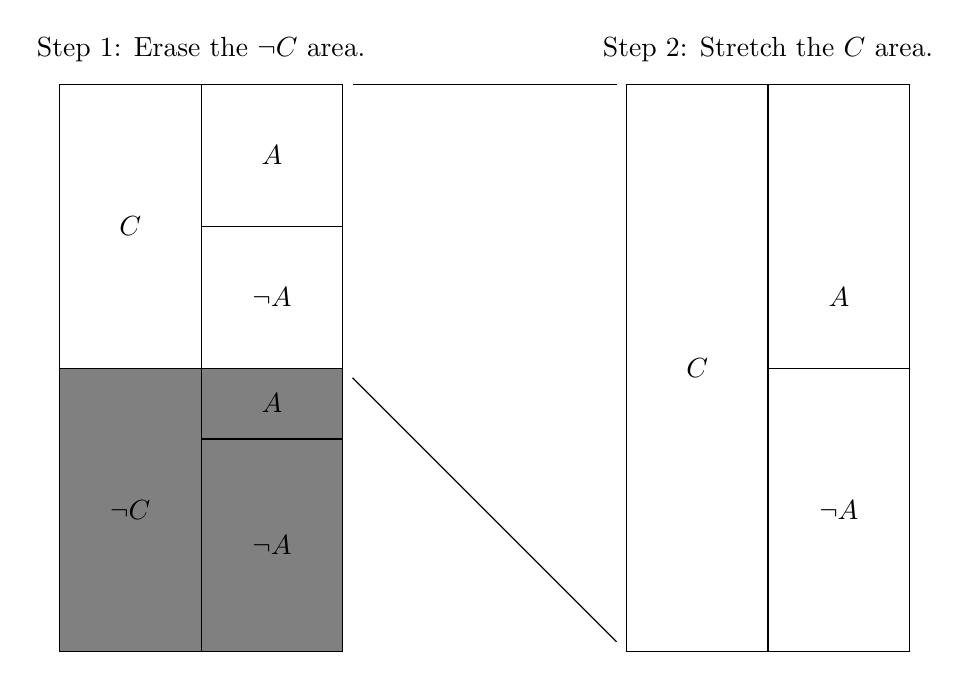
\begin{tikzpicture}[scale=.9]

\draw(2,8.5) node {Step 1: Erase the $\neg C$ area.};

\draw(4, 8) node (a){};

\draw (4, 4) node (b){};

\fill[gray] (0, 0) rectangle (4, 4);


\draw (0,0) rectangle (4, 8);

\draw (2, 0) -- (2, 8);

\draw (2, 6) -- (4, 6);

\draw (0, 4) -- (4, 4);

\draw (2, 3) -- (4, 3);

\draw (1, 6) node {$C$};

\draw (1, 2) node {$\neg C$};

\draw (3, 7) node {$A$};

\draw (3, 5) node {$\neg A$};

\draw (3, 3.5) node {$A$};

\draw (3, 1.5) node {$\neg A$};



\begin{scope}[xshift=8cm]

\draw (0, 8) node (c){};
\draw (0, 0) node (d){};
\draw(2,8.5) node {Step 2: Stretch the $C$ area.};

\draw (0,0) rectangle (4, 8);

\draw (2, 0) -- (2, 8);

\draw (2, 4) -- (4, 4);


\draw (1, 4) node {$C$};


\draw (3, 5) node {$A$};

\draw (3, 2) node {$\neg A$};
\end{scope}

\draw (a) -- (c);
\draw (b) -- (d);

\end{tikzpicture}
\caption{Calculating conditional probability}
\label{fig-conditional-prob}

\end{figure}

\autoref{fig-conditional-prob} shows how to calculate the probability of $A$ conditional on $C$ by erasing the bottom half of the diagram, and stretching out the remaining part of the rectangle so its height is 1 (in effect multiplying the height of each of its sub-regions by $\frac{1}{Pr(C)}$).  The new height of the $A$ region is $Pr(A|C)$.

\begin{figure}
\centering
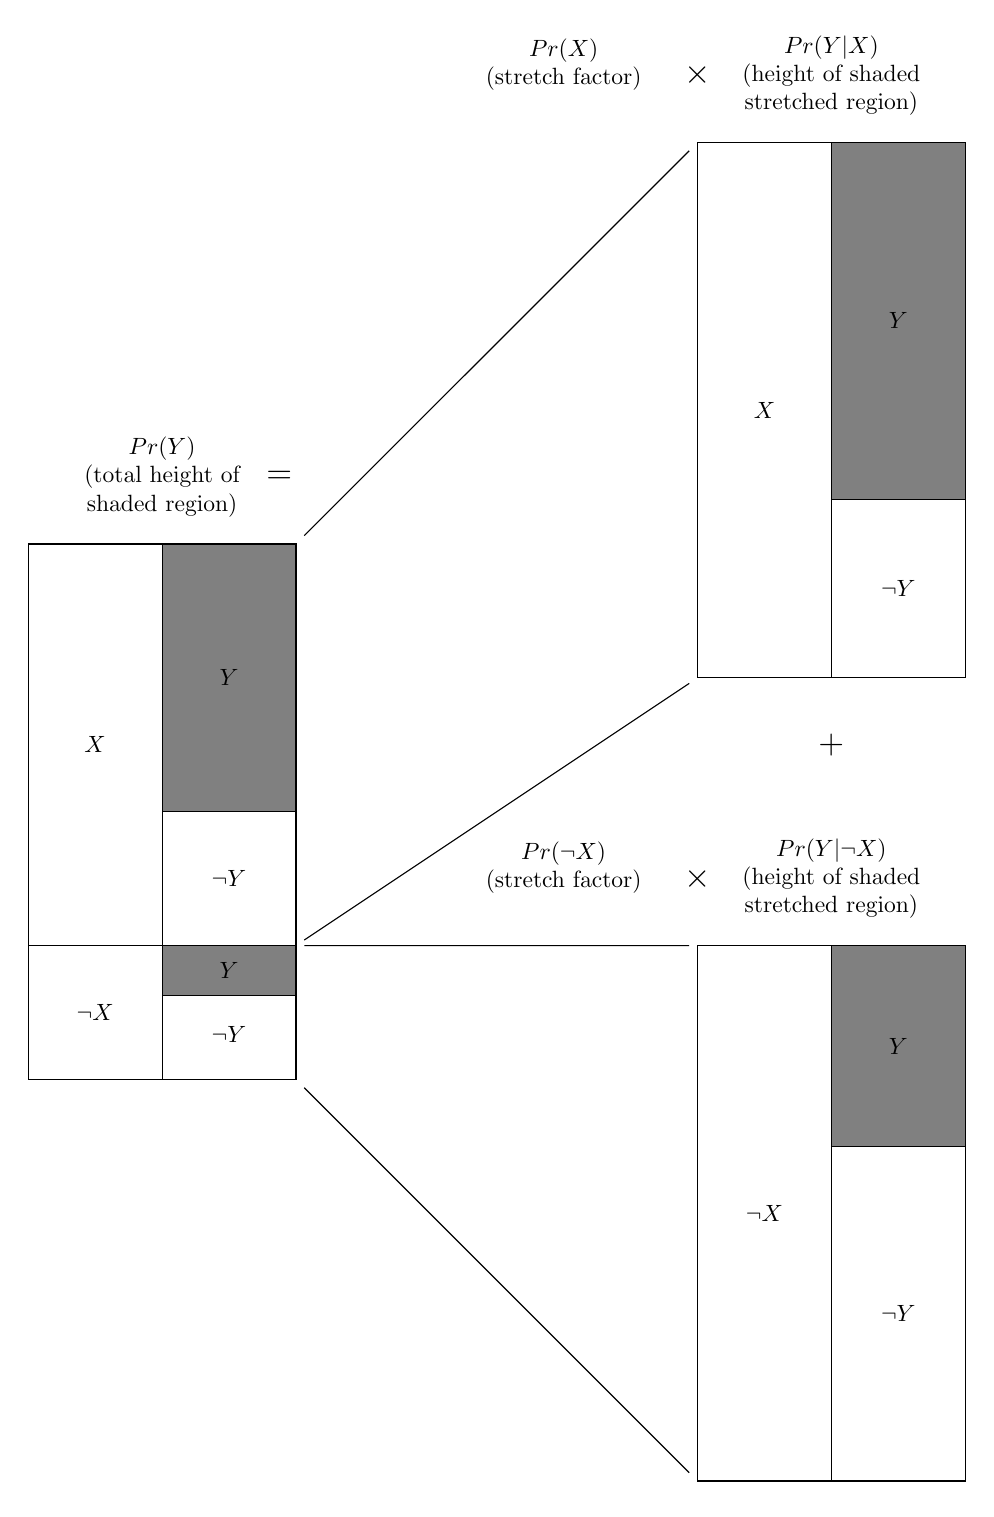
\begin{tikzpicture}[scale = 0.85, every node/.style={scale=0.85}]

\draw (4, 8) node (a){};
\draw (4, 2) node(b){};
\draw (4, 0) node(c){};

\draw(2,9) node [align =center]{$Pr(Y)$\\ (total height of\\shaded region)};

\draw (3.75, 9) node {\Large{=}};

\fill[gray] (2, 4) rectangle (4, 8);

\fill[gray] (2, 1.25) rectangle (4, 2);

\draw (0,0) rectangle (4, 8);

\draw (2, 0) -- (2, 8);

\draw (2, 4) -- (4, 4);

\draw (0, 2) -- (4, 2);

\draw (2, 1.25) -- (4, 1.25);

\draw (1, 5) node {$X$};

\draw (1, 1) node {$\neg X$};

\draw (3, 6) node {$Y$};

\draw (3, 3) node {$\neg Y$};

\draw (3, 1.625) node {$Y$};

\draw (3, 0.675) node {$\neg Y$};



\begin{scope}[xshift=10cm, yshift=6cm]

\draw (0, 8) node(a1){};
\draw (0, 0) node(b1){};
\draw(2,9) node[align =center] {$Pr(Y|X)$\\(height of shaded\\stretched region)};

\draw(-2,9) node[align =center] {$Pr(X)$\\(stretch factor)\\~};

\draw (0, 9) node{\Large{$\times$}};

\fill[gray] (2, 2.667) rectangle (4, 8);

\draw (0,0) rectangle (4, 8);

\draw (2, 0) -- (2, 8);

\draw (2, 2.667) -- (4, 2.667);


\draw (1, 4) node {$X$};


\draw (3, 5.333) node {$Y$};

\draw (3, 1.333) node {$\neg Y$};

\draw (2, -1) node {\Large{$+$}};
\end{scope}

\begin{scope}[xshift=10cm, yshift= -6cm]
\draw(0, 8) node (b2){};
\draw(0, 0) node (c2){};
\draw(2,9) node[align =center] {$Pr(Y|\neg X)$\\(height of shaded\\stretched region)};

\draw(-2,9) node[align =center] {$Pr(\neg X)$\\(stretch factor)\\~};

\draw (0, 9) node{\Large{$\times$}};

\fill[gray] (2, 5) rectangle (4, 8);

\draw (0,0) rectangle (4, 8);

\draw (2, 0) -- (2, 8);

\draw (2, 5) -- (4, 5);


\draw (1, 4) node {$\neg X$};


\draw (3, 6.5) node {$Y$};

\draw (3, 2.5) node {$\neg Y$};
\end{scope}

\draw (a) -- (a1);
\draw (b) -- (b1);
\draw (b) -- (b2);
\draw (c) -- (c2);

\end{tikzpicture}
\caption{The Law of Total Probability}
\label{fig-total-prob}
\end{figure}


According to the Law of Total Probability (illustrated in \autoref{fig-total-prob}), for any two propositions $X$ and $Y$,
%
\begin{equation}
\label{eq-total-probability}
Pr(Y) = Pr(Y|X)\times Pr(X) + Pr(Y|\neg X) \times Pr(\neg X).
\end{equation}

Consider any two propositions $A$ and $C$ such that $P(A \wedge C) > 0$, and $P(A \wedge \neg C) > 0$.  Plugging in $A$ for $X$ and $A \rightarrow C$ for $Y$ in \autoref{eq-total-probability} yields:
%
\begin{equation}
\label{eq-crucial-instance}
Pr(A \rightarrow C) = Pr(A \rightarrow C|C)\times Pr(C) + Pr(A \rightarrow C|\neg C) \times Pr(\neg C).
\end{equation}
%
In other words, we can split the probability space into a $C$ part and a $\neg C$ part, and figure out the probability of $A \rightarrow C$ by averaging its probabilities conditional on each part, a procedure illustrated in \autoref{fig-triviality}.  Consider the probability distribution $Pr_C$ such that for all propositions $X$, $Pr_C(X) = Pr(X|C)$ (shown in the top center of \autoref{fig-triviality}). Using the fact that $Pr_C(A) >0$, the fact that $Pr_C(C) =1$, and the definition of conditional probability, we can show that
%
\begin{equation}
\label{eq-double-conditional-positive}
Pr_C(C|A) =1.
\end{equation}
%
Thus, by \textsc{the thesis} and \autoref{eq-double-conditional-positive},
%
\begin{equation}
\label{eq-single-positive}
Pr_C(A\rightarrow C) = 1.
\end{equation}
%
By the definition of $Pr_C$ and \autoref{eq-single-positive},
%
\begin{equation}
\label{eq-if-c}
Pr(A \rightarrow C| C) = 1.
\end{equation}

Likewise, when we consider the probability distribution $Pr_{\neg C}$ such that for all $X$, $Pr_{\neg C}(X) = Pr(X|\neg C)$ (shown in the bottom center of \autoref{fig-triviality}), we see by the fact that $Pr_C(A) >0$, the fact that $Pr_C(C) =1$, and the definition of conditional probability that
%
\begin{equation}
\label{eq-double-conditional-negative}
Pr_{\neg C}(C|A) = 0.
\end{equation}
%
Thus, by \textsc{the thesis}, and \autoref{eq-double-conditional-negative},
%
\begin{equation}
\label{eq-single-negative}
Pr_{\neg C}(A \rightarrow C) = 0.
\end{equation}
%
And by the definition of $Pr_{\neg C}$ and \autoref{eq-single-negative},
\begin{equation}
\label{eq-if-not-c}Pr(A \rightarrow C|\neg C) = 0.
\end{equation}
%
Using \autoref{eq-if-c} and \autoref{eq-if-not-c} to make the appropriate substitutions into equation \autoref{eq-crucial-instance}, we get:
%
\begin{equation}
\label{eq-almost-there}
Pr(A \rightarrow C) = 1 \times Pr(C) + 0 \times Pr(\neg C) = Pr(C).
\end{equation}
%
But by \textsc{the thesis},
%
\begin{equation}
Pr(A \rightarrow C) = Pr(C|A).
\end{equation}
%
Substituting $Pr(C|A)$ for $Pr(A \rightarrow C)$ on the left-hand side of \autoref{eq-almost-there}, we get:
%
\begin{equation}
\label{eq-independent}
Pr(C|A) = Pr(C)
\end{equation}
%
---in other words, $A$ and $C$ are probabilistically independent.

The above proof shows that \autoref{eq-independent} holds for arbitrary propositions $A$ and $C$, provided both $Pr(A \wedge C)$ and $Pr(A \wedge \neg C)$ are both greater than 0.  Therefore \autoref{eq-independent} should hold for all pairs of propositions $A$ and $C$ such that $Pr(A \wedge C)$ and $Pr(A \wedge \neg C)$ are both greater than 0.  But this is only possible in trivial probability spaces.  So one of our assumptions must have gone wrong, and the natural place to pin the blame is on \textsc{the thesis}.

\begin{figure}
\begin{tikzpicture}[scale = 0.75, every node/.style={scale=0.85}]

\draw(4, 8) node (a){};
\draw (4, 4) node (b){};
\draw (4, 0) node (c){};

\draw (0,0) rectangle (4, 8);

\draw (2, 0) -- (2, 8);

\draw (2, 6) -- (4, 6);

\draw (0, 4) -- (4, 4);

\draw (2, 3) -- (4, 3);

\draw (1, 6) node {$C$};

\draw (1, 2) node {$\neg C$};

\draw (3, 7) node {$A$};

\draw (3, 5) node {$\neg A$};

\draw (3, 3.5) node {$A$};

\draw (3, 1.5) node {$\neg A$};

\begin{scope}[xshift=6cm, yshift=6cm]
\draw (2, 8.5) node {$Pr_{C}(A \rightarrow C) = 1$};


\draw (0, 8) node (a1){};
\draw (0, 0) node (b1){};

\draw (0,0) rectangle (4, 8);

\draw (2, 0) -- (2, 8);

\draw (2, 4) -- (4, 4);


\draw (1, 4) node {$C$};


\draw (3, 5) node {$A$};

\draw (3, 2) node {$\neg A$};

\draw (4, 8) node(d1){};
\draw(4, 4) node(e1){};

\begin{scope}[xshift = 6cm]
\draw (2, 8.5) node {$Pr_C(C|A) = 1$};

\draw (0,0) rectangle (4, 8);
\draw (2, 8) -- (2, 0);
\draw (1, 4) node {$C$};
\draw (3, 4) node {$A$};
\draw (0, 8) node(d3){};
\draw (0, 0) node (e3){};
\end{scope}

\end{scope}

\begin{scope}[xshift=6cm, yshift=-6cm]
\draw (2, 8.5) node {$Pr_{\neg C}(A \rightarrow C) = 0$};

\draw (0, 8) node (b2){};
\draw (0, 0) node (c2){};

\draw (0,0) rectangle (4, 8);

\draw (2, 0) -- (2, 8);

\draw (2, 6) -- (4, 6);


\draw (1, 4) node {$\neg C$};


\draw (3, 7) node {$A$};

\draw (3, 3) node {$\neg A$};

\draw (4, 8) node (d2){};
\draw (4, 6) node (e2){};

\begin{scope}[xshift = 6cm]
\draw (2, 8.5) node {$Pr_{\neg C}(C|A) = 0$};
\draw (0,0) rectangle (4, 8);
\draw (2, 8) -- (2, 0);
\draw (1, 4) node {$\neg C$};
\draw (3, 4) node {$A$};
\draw (0, 8) node(d4){};
\draw (0, 0) node (e4){};
\end{scope}
\end{scope}

\draw (a) -- (a1);
\draw (b) -- (b1);
\draw (b) -- (b2);
\draw (c) -- (c2);
\draw (d1) -- (d3);
\draw (e1) -- (e3);
\draw (d2) -- (d4);
\draw (e2) -- (e4);
\end{tikzpicture}
\caption{The Lewis triviality theorem illustrated}
\label{fig-triviality}
\end{figure}

There are various possible ways out of Lewis's triviality theorem.  The proof assumes that the conditional $A \rightarrow C$ has a single set of truth conditions, which remain stable across $Pr$, $Pr_C$, and $Pr_{\neg C}$.  Defenders of \textsc{the thesis} might reject this assumption and claim that the truth-conditions of conditionals are context-dependent.  The proof also assumes that \textsc{the thesis} holds for all probability functions and all conditionals.  Defenders of \textsc{the thesis} might retreat and claim that it is true for only some conditionals, or some probability functions.

Unfortunately, both escape routes are treacherous.  New triviality theorems can be derived from much weaker assumptions; for a helpful survey, see \citet{hall-hajek}.  There are even triviality results that use non-probabilistic variants of \textsc{the thesis} \citep{gardenfors-knowledge}, and trivializing versions of \textsc{the thesis} that apply to counterfactuals rather than indicatives \citep{williams-counterfactual-triviality}. On a slightly more optimistic note, \emph{non}-triviality results can be obtained by adopting (sufficiently weak) non-classical logics \citep{morgan-mares-nontrivial}.

Another way out of Lewis's triviality theorem is to reject \textsc{the thesis}.  \citet{kaufmann-grain} produces examples of indicative conditionals in English that intuitively seem to violate \textsc{the thesis}, and \citet{douven-verbrugge} provide experimental evidence that English speakers' judgments about indicative conditionals violate \textsc{the thesis}.

If probability is probability of truth, defenders of the NTV view should reject \textsc{the thesis} too.  However, defenders of the NTV view typically defend versions \textsc{the thesis}, but adopt alternative interpretations of `probability', on which the probability of a conditional is not the probability of its truth.

Calling on alternative theories of probability makes sense: probability is a versatile explanatory tool, and the NTV theory has plenty of explaining to do.  In particular, the NTV theory needs to explain why conditionals seem to have the features of truth-evaluable statements.  It is sometimes reasonable to believe a conditional---but ordinarily, to believe something is to believe that it is true.  Likewise, it is sometimes reasonable to assert a conditional---but ordinarily, to assert something is to claim that it is true.  Arguments with conditionals in their premises and conclusions are sometimes valid and sometimes invalid---but ordinarily, a valid argument is one that cannot have true premises and a false conclusion, and it's not clear how to fruitfully apply the concept of validity when a premise or conclusion lacks truth conditions altogether.

\citet{Adams1975-ADATLO-4} and \citet{Edgington1986-EDGDCH} give a probabilistic account of belief in conditionals.  Belief comes in degrees, which are measured by probabilities.  A person's degree of belief in a conditional is simply her conditional degree of belief in its consequent on its antecedent.

\citet{Adams1975-ADATLO-4} gives a probabilistic account of validity for conditionals.  An argument is said to be probabilistically valid just in case it is impossible for its premises to be probable and its conclusion improbable.  More precisely, an argument from premises $P_1, P_2,\ldots, P_n$ to conclusion $C$ is valid just in case, for every real number $\epsilon > 0$, there is a real number $\delta > 0$ such that, if each of $P_1, P_2,\ldots, P_n$ has probability greater than $1-\delta$, then $C$ has probability at least $1-\epsilon$.

Adams' definition of validity coincides with the classical definition where $P_1, P_2,\ldots, P_n$ and $C$ are conditional-free sentences, and lets us define validity for arguments containing simple conditionals.  The theory is built to handle only simple conditionals, and does not let us assess validity for arguments containing compound sentences with conditionals as parts.  \citet{McGee1989-MCGCPA} extends Adams' theory to cover compounds of conditionals.

\citet{edgington-conditionals} gives a non-probabilistic account of what it is to assert a conditional: it is to assert the consequent if the antecedent is true, and to assert nothing otherwise.  She argues that her account assimilates conditional assertions to a larger class of conditional speech acts, including:
\begin{description}
\item[Conditional Questions] `If he phones, what shall I say?'
\item[Conditional Commands] `If he phones, hang up.'
\item[Conditional Promises] `If he phones, I promise not to be rude.'
\item[Conditional Agreements] `If he phones, we're on for Sunday.'
\item[Conditional Offers] `If you phone, you can have a 20\% discount.'
\end{description}
Any speech act whatsoever, she claims, can be performed conditionally or unconditionally.  We can think of conditionals as `speech act bombs' primed to detonate when and only when the antecedent is true \citep[see][]{Egan2009-EGABBA}.



\section{Dynamic Semantics}

So far, we've seen several accounts of conditionals that posit more to their meanings than truth conditions---either because conditionals have no truth conditions (on the NTV account) or because their truth conditions are not sufficient to determine when they can reasonably be asserted (on the material conditional account).  Enter dynamic semantics, which provides new tools for modeling meaning.

Dynamic semantics explains the meanings of sentences by appeal to a \emph{conversational context}---a set of background assumptions taken for granted by all the participants in a conversation.  For instance, if a group of friends is discussing where to go for lunch, the conversational context might include the information that among the nearby restaurants are Veggie Garden and Buddha's Palace.  The \emph{context set} is a set of worlds compatible with those background assumptions \citep[see][84]{stalnaker-assertion}.\footnote{To give a complete theory of conditionals, the conversational context will need to include more information than just the context set.  Other proposed parameters include a probability function or set of probability functions \citep{yalcin-epistemic, yalcin-bayesian}, and a function that ranks worlds from most to least likely \citep{spohn-ranking}.  However, I focus my exposition on the context set to provide a simple illustration of the main ideas.}

The conversational context changes as the conversation progresses, and the context set shrinks and grows accordingly.  When a participant makes an assertion, then the content of the assertion is added to the context, and all the worlds incompatible with what is asserted are eliminated from the context set.  For instance, if someone asserts that Veggie Garden is open, then the worlds where Veggie Garden is closed are eliminated from the context set.

\autoref{fig-context-set} depicts the effect of asserting `Veggie Garden is open today' on the context set.  The original context set is shown in the rectangle at the top of the figure: the circles depict worlds.  Each world is labeled with a set of propositions true at that world: `BP' stands for `Buddha's Palace is open'; `VG' stands for `Veggie Garden is open'; and `TD' stands for `we can get gluten-free tofu dogs'.

\begin{figure}
\centering
\begin{subfigure}{\textwidth}
\centering
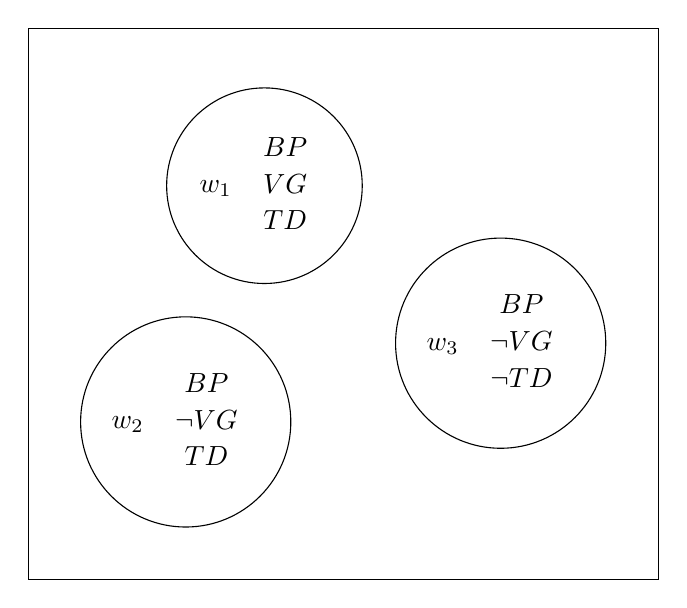
\begin{tikzpicture}

\draw(-2, 0) rectangle (6, 7);

\draw (1, 5) node [align =center, circle, draw] {$w_1$ \begin{tabular}{c}$BP$\\$VG$\\$TD$\end{tabular}};

\draw (0, 2) node [align =center, circle, draw] {$w_2$ \begin{tabular}{c}$BP$\\$\neg VG$\\$TD$\end{tabular}};

\draw (4, 3) node [align =center, circle, draw] {$w_3$ \begin{tabular}{c}$BP$\\$\neg VG$\\$\neg TD$\end{tabular}};

\end{tikzpicture}
\caption{The original context set}
\label{fig-original-context}
\end{subfigure}

\begin{subfigure}{\textwidth}
\centering
\begin{tikzpicture}

\draw(-2, 0) rectangle (6, 7);

\draw (1, 5) node [align =center, circle, draw] {$w_1$ \begin{tabular}{c}$BP$\\$VG$\\$TD$\end{tabular}};

\end{tikzpicture}
\caption{The context set after an assertion of `Veggie Garden is open'}
\label{fig-assertion}
\end{subfigure}

\caption{The effects of an assertion on the context set}
\label{fig-context-set}
\end{figure}

Notice that some assertions have no effect on the context set.  If someone were to assert `Buddha's Palace is open', none of the worlds in the context set would be eliminated.  This is because `Buddha's Palace is open' is already acceptable in the original context---it follows from what is accepted.

\citet{Starr2014-STAAUT-2} proposes that within this dynamic semantics framework, conditionals can be understood as \emph{tests}, along the lines of the Ramsey test.  To determine the effect of asserting a conditional `if $A$, then $B$' on a context $c$, we first suppose $A$, by considering the context $c[A]$ that results from adding $A$ to $c$.  We then check whether $B$ is true under the supposition.  If $B$ is true at $c[A]$, then $c$ `passes' the test, and $c$ remains unchanged.  Otherwise, $c$ `fails' the test.  If a conditional passes the test, it is acceptable in the original context.

This characterization of acceptability, by itself, is not enough to determine the effect of uttering a conditional in a context where it is not already acceptable.  For instance, suppose you go to pet a dog, and I say `if you pet it, it will bite.'  This conditional doesn't follow from our shared background information, but you can use it to rule out possibilities---in particular, those possibilities where you pet the dog and it does not bite.  What explains the relationship between my utterance and the corresponding change to the context set?  In very broad terms, uttering a conditional should change the context set so that the conditional becomes acceptable, and the change involved should be the smallest one that does the job.  There are multiple ways of spelling out what constitutes a minimal change to contextual information, but the part of the account that deals with acceptability can be separated from the part that deals with context change.

To illustrate the concept of a conditional test, consider the conditional `if Veggie Garden is open, then we can get gluten-free tofu dogs', as asserted in the context depicted by \autoref{fig-original-context}.  To perform the test, we first create a new context, by augmenting the old context with the information that Veggie Garden is open; the resulting context set is depicted in \autoref{fig-assertion}.  We then check whether, in the new context, `we can get gluten-free tofu dogs' is acceptable.  If so, the old context passes the test, and the conditional is acceptable in the old context; otherwise, the old context fails the test, and the conditional is not acceptable in the old context. Starr extends his account to handle counterfactuals (which use a modified test in which the context set is expanded with extra possibilities before adding the information in the antecedent).

Other theorists offer context-dependent truth conditions for conditionals using the tools of dynamic semantics. \citet{stalnaker-indicative} and \citet{Williams2008-WILCAC-2} defend a modified closest-worlds theory of indicative conditionals, where, if $w$ is a world in the context set, every world in the context set is stipulated to be closer to $w$ than every world outside it. \citet{Gillies2007-GILCS} and \citet{fintel-dynamic} propose strict conditional theories of counterfactuals, where a set of salient worlds is fixed by the context.  New worlds are added to the set as the conversation goes on; in particular, if someone asserts a conditional whose antecedent is false at all the salient worlds, the set is expanded to include at least one world compatible with the antecedent.


\section{Conditionals as Modal Restrictors}

According to \citet[86]{kratzer-2012}, many of the above views of conditionals are `based on a momentous syntactic mistake.'  Contrary to popular opinion, she claims, `There is no two-place \emph{if\ldots then} connective in the logical forms for natural languages.'  Instead, conditionals restrict modal operators.

One can think of modal operators as quantifiers over possible worlds: to say that necessarily $2+2 = 4$ is to say that in all possible worlds, $2+2=4$; to say that possibly pigs fly is to say that in some possible world, pigs fly; and to say that it will probably rain is to say that in most possible worlds (on some suitable way of measuring `most'), it rains.  Like quantifiers, modal operators can be restricted.  To say that necessarily, if the Peano axioms are true, then $2+2=4$, is to say that in all possible worlds where the Peano axioms are true, $2+2=4$.  Likewise, to say that if pigs had hollow bones, then possibly pigs would fly, is to say that in some possible world where pigs have hollow bones, pigs fly, and to say that if there are cumulus clouds on the horizon, it will probably rain, is to say that in most possible worlds where there are cumulus clouds on the horizon, it will rain.

The modal restrictor view is a generalization of work by  \citet{lewis-adverbs} who notes that conditionals can be used to restrict quantifiers.  Consider the following class of examples.
\begin{quote}
\begin{tabular}{ll}
Sometimes\\
Always\\
Usually\\
Never
\end{tabular}
 if a farmer owns a donkey, she feeds it carrots.
\end{quote}
The quantifiers `sometimes', `always', `usually', and `never' are what Lewis calls \emph{unselective quantifiers}.  To say that always, farmers feed donkeys carrots is to say that for all ways of assigning a farmer to $x$ and a donkey to $y$, $x$ feeds $y$ carrots.  To add the clause `if a farmer owns a donkey' is to restrict the quantifier, so that it ranges only over cases where farmer $x$ owns donkey $y$.

The modal restrictor view is Y-shaped: it can handle both indicatives and counterfactuals \citep{kratzer-notional-modality}.  To explain how this works, we need three ingredients: a modal base, the modal force of an operator, and an ordering.

According to Kratzer, the context of an utterance supplies a \emph{modal base}, or a function $f$ mapping each world $w$ to a set of propositions that is `held fixed' when we speculate about what might or must have been true at $w$.   When we consider what is physically possible, the modal base might assign to each world the laws of physics that obtain at that world, but leave out physically contingent truths.  When a detective speculates about who the burglar might be, the modal base might assign to each world the detective's evidence at that world.  To determine what is possible (or necessary, or likely) at a world $w$, we need to quantify over the possible worlds where the all of the propositions in $f(w)$ are true.\footnote{Kratzer's theory could be reformulated in terms of a familiar two-place accessibility relation among worlds. We might say that world $x$ is accessible from world $w$ ($Rwx$ in the usual formalism) if and only if  all of the propositions in $f(w)$ are true at $x$.   A few complications arise when the modal base maps some worlds onto inconsistent sets of propositions.   Kratzer wants to say that in such cases, there are non-trivial facts about what is possible; she gives the example of a modal base that assigns to each world the set of propositions that are required by a group of Maori elders in that world \citep[16-20]{kratzer-notional-modality}.  In one world $w$, the elders disagree amongst themselves, and so their requirements are inconsistent.  Nonetheless, there are non-trivial facts about what is necessary at $w$ according to the elders' requirements; Kratzer claims that the structure of the set $f(w)$ of propositions plays an essential role in determining what is necessary.}

Different operators are associated with different kinds of \emph{modal force}---roughly, different kinds of quantification over possible worlds.  The operators `necessarily', `possibly', `it is likely that', and `it is a good possibility that' are all associated with different modal forces.  Finally, the context of utterance supplies an \emph{ordering source} $g$, which lets us map each world to an ordering over worlds.\footnote{Kratzer's ordering source officially maps worlds to sets of propositions, which are then used to create an ordering.  I omit this extra step.}  (One possible interpretation of this ordering is the `closeness' ordering from \autoref{closest}, but there are others.  Conditional and unconditional statements about what ought to happen use an ordering source that ranks worlds from most to least ideal.)

We can then say that the conditional `Necessarily if $A$, then $B$' is true at a world $w$ just in case $B$ is true at all the closest $A$-worlds to $w$ (according to the ordering $g(w)$) where all the propositions in $f(w)$ are true.  Likewise,  `Possibly if $A$, then $B$' is true at a world $w$ just in case at some of the closest $A$-worlds to $w$ (according to the ordering $g(w)$) where all the propositions in $f(w)$ are true, and similarly for other operators with other modal force.  For indicative conditionals, the modal base is some piece of salient known information.  For counterfactual conditionals, the modal base is empty (and thus, all possible worlds are consistent with it) while the ordering source is very rich.  Kratzer's account even has the material conditional account as a special case, where the modal base maps each world $w$ to a set of propositions true only at $w$, and the strict conditional as another special case, where the modal base is empty and the ordering source is completely noncommittal, invariably ranking all worlds on a par with each other.

`Bare' conditionals cause trouble for the modal restrictor view.  Conditionals supposedly restrict modal operators, but where is the modal operator in a conditional like `If the lights in his study are on, then Roger is home'?   \citet{kratzer-conditional-necessity, kratzer-notional-modality} argues that conditionals without overt modal operators nonetheless contain implicit modal operators; the underlying logical form of the example conditional is `(MUST: the lights in his study are on) Roger is home'; the epistemic `MUST' is unspoken.

\citet{heim-thesis} provides evidence for Kratzer's modalized interpretation of bare conditionals in the form of `donkey sentences' like `If John owns a donkey, then he feeds it carrots'.  On at least one plausible reading, our sample donkey sentence means that John feeds carrots to every donkey he owns---or in more cumbersome terms, for every $x$ such that $x$ is a donkey and John owns $x$, John feeds $x$ carrots.  If the conditional were an ordinary two-place connective, we would have trouble explaining how the same variable $x$, bound by the same quantifier, could occur in both the antecedent and the consequent of the donkey sentence.  The conditional would have the form $A \rightarrow B$, where $A$ contained a quantifier ranging over donkeys.  But Kratzer's restrictor analysis, together with the assumption that bare conditionals contain a tacit necessity operator, gives the correct reading, while providing a uniform treatment of bare and modalized conditionals.

It is often claimed that Kratzer's modal restrictor theory allows us to escape the triviality results of \autoref{ntv}. \citet{rothschild-kratzer}, for instance, suggests that Kratzer can escape the triviality results by denying \textsc{the thesis}.  To illustrate Rothschild's argument, let's consider the conditional I originally used to motivate \textsc{the thesis}.
\begin{description}
\item[ACE] If I draw a red ace, then it will be the ace of hearts.
\end{description}
I accept the conditional:
\begin{description}
\item[CHANCY ACE] With probability $1/2$, if I draw a red ace, then it will be the ace of hearts.
\end{description}
Rothschild suggests that on Kratzer's account, \textsc{chancy ace} does not express the thought that \textsc{ace} has probability $1/2$, or the thought that the probability of \textsc{ace}'s being true is $1/2$.  When I assert \textsc{chancy ace}, I am not asserting that \textsc{ace} has probability $1/2$.  Furthermore, when I am 50\% confident that if I draw a red ace, it will be the ace of hearts, this does not amount to my being 50\% confident that \textsc{ace} is true.

 \citet{charlow-trivial} argues that even if Rothschild is right, Kratzer's account is still vulnerable to the triviality result, since \autoref{eq-if-c} and \autoref{eq-if-not-c} can be motivated independently of \textsc{the thesis}.  He goes on to argue that other easy ways out of the triviality result fail on the modal restrictor view.

 
\section{Conclusion}

Conditionals are important in both everyday reasoning and philosophical argument.  There are conditional beliefs, conditional assertions, and conditional propositions, all of which can figure in arguments.  The theories canvassed in this article try to systematize the broad range of data about which conditionals seem true, and which inferences seem valid.  More phenomena remain to be explained: this article has focused on conditional beliefs and assertions, and on conditionals in English.

We can gather the similarities among the accounts discussed above into a sort of rake-shaped theory (a generalization of Bennett's concept of a Y-shaped theory), with a short `handle' that captures what is common to all conditionals, which then splits into many `tines' that capture the particularities of individual theories.  All of the theories we have considered so far have the following commitments in common.
\begin{enumerate}
\item Conditionals are evaluated at `points'.

\item To evaluate a conditional `if $A$, then $C$' at a point $p$, one generates a new point $q$ by adding the information in $A$ to $p$.

\item The evaluation of the consequent $C$ at $q$ is the evaluation of the entire conditional at $p$.
\end{enumerate}
The accounts disagree about the natures of points, what status conditionals and their consequents should be evaluated for, and what adding an antecedent amounts to.  \autoref{table:rake} summarizes how different views answer this question. (NB: Selection function and relevant logic accounts typically treat the initial point and the new point as belonging to different types---the initial point is a world, while the new point is a set of worlds. But we can ensure that both points are of the same type by rewriting the theory so that the initial point is a singleton set of one world; this is what I have done in \autoref{table:rake}.)

\noindent
\bgroup
\def\arraystretch{1.1}
\setlength\tabcolsep{.8em}
\begin{sidewaystable}[pht!]
\centering
\begin{tabular}{p{0.19\textheight}p{0.15\textheight}p{0.25\textheight}p{0.27\textheight}}

    & Points & Status & Adding $A$ to a Point\\

\hline\hline

\textsc{Strict Conditional} &
	Sets of worlds &
	Truth in all worlds (original point is a singleton $\{w\}$) &
	Taking all worlds possible at $w$ compatible with $A$\\
\textsc{Closest Worlds and Past Predominance} &
    Sets of worlds &
	Truth in all worlds (original point is a singleton $\{w\}$) &
	Taking all closest worlds possible at $w$ compatible with $A$\\
\textsc{Causal Modeling} &
	\raggedright Causal models with valuations &
	Truth in a model &
	Intervening to make $A$ true\\
\textsc{Relevant Logic} &
	Sets of worlds &
	Truth in all worlds (original point is a singleton $\{w\}$) &
	Taking all worlds $y$ such that $Rwxy$ for some world $x$ compatible with $A$\\
\textsc{Material Conditional} &
	Worlds &
	Truth in the world &
	Doing nothing if $A$ is true; moving to the `absurd world' (where everything is true) otherwise\\
\textsc{Probability Accounts} &
    \raggedright Probability functions &
	Probability $x \in [0, 1]$ &
	Conditionalizing on $A$\\
\textsc{Dynamic Test Theory} &
	Contexts &
	Acceptability &
	Updating to accommodate an assertion of $A$\\
\textsc{Modal Restrictors} &
	Information states: modal base + ordering source &
	Obtaining with a given modal force &
	Taking all closest worlds to $A$ in the modal base, according to the ordering source\\
\end{tabular}
\caption{Theories of conditionals and their components}
\label{table:rake}
\end{sidewaystable}
\egroup

Within each of the accounts, there are open questions: the nature of the selection function; the correct interpretation of counterpossibles; how best to respond to the triviality theorems; what makes a conditional believable or assertable in a given context; how to handle bare modals on the restrictor account.

There are also open questions about how the accounts interact.  Some accounts seem to be special cases of others: the past predominance view is a way of filling in the meaning of `closest' on the closest-worlds account.  At other times, different accounts appear to be rivals: it can't be both that indicative conditionals have the truth conditions given by the material interpretation, and that they lack truth values.  At other times, they seem to be modeling different domains: as with Pearl's causal modeling theory of counterfactuals and Starr's dynamic semantics theory of indicatives.  Much of the interest for future research lies in understanding the interactions between the different models of conditionals.

If conditionals are useful in a wide variety of domains, from childhood development to everyday reasoning to philosophy, then conditionals are well worth studying.  I have given reasons for thinking that conditionals are useful in a wide variety of domains.  You may draw your own conclusions.